% ============================================================================
%  biosim-lab — "How it actually works", for people who are not experts.
%  Build:  xelatex main.tex  (twice, for the table of contents)
%  Licence: MIT, same as the code.
% ============================================================================
\documentclass[11pt,a4paper]{article}

\usepackage{fontspec}
\setmainfont{STIX Two Text}
\setsansfont{Helvetica Neue}[Scale=MatchLowercase]
\setmonofont{Menlo}[Scale=0.86]
\usepackage{unicode-math}
\setmathfont{STIX Two Math}

\usepackage[margin=2.4cm,top=2.2cm,bottom=2.4cm]{geometry}
\usepackage{amsmath}
\usepackage{graphicx}
\usepackage{booktabs}
\usepackage{array}
\usepackage{xcolor}
\usepackage{tcolorbox}
\usepackage{tikz}
\usepackage{pgfplots}
\usepackage{siunitx}
\usepackage{enumitem}
\usepackage{microtype}
\usepackage{caption}
\usepackage[hidelinks,bookmarksnumbered]{hyperref}
\usepackage{fancyhdr}

\pgfplotsset{compat=1.18}
\usetikzlibrary{arrows.meta,positioning,decorations.pathmorphing,decorations.markings,
                patterns,calc,shapes.geometric,fit,backgrounds}
\tcbuselibrary{skins,breakable}

\definecolor{blue1}{HTML}{2A78D6}
\definecolor{orange1}{HTML}{EB6834}
\definecolor{aqua1}{HTML}{1BAF7A}
\definecolor{red1}{HTML}{E34948}
\definecolor{ink}{HTML}{0B0B0B}
\definecolor{muted}{HTML}{52514E}
\definecolor{rule1}{HTML}{E6E5E1}
\definecolor{surface}{HTML}{FCFCFB}

\captionsetup{font=small,labelfont={bf,color=muted},textfont={color=muted}}
\setlist{itemsep=2pt,topsep=4pt,parsep=0pt}
\sisetup{per-mode=symbol,detect-all}

\pagestyle{fancy}\fancyhf{}
\renewcommand{\headrulewidth}{0.4pt}
\fancyhead[L]{\footnotesize\sffamily\color{muted}biosim-lab — how it works}
\fancyhead[R]{\footnotesize\sffamily\color{muted}\thepage}

% --- boxes ------------------------------------------------------------------
\newtcolorbox{plain}[1][]{
  enhanced, breakable, colback=blue1!5, colframe=blue1!55, boxrule=0.6pt,
  arc=2pt, left=8pt, right=8pt, top=6pt, bottom=6pt,
  fonttitle=\sffamily\bfseries\small, coltitle=blue1!75!black,
  title={In plain English}, #1}

\newtcolorbox{analogy}[1][]{
  enhanced, breakable, colback=aqua1!6, colframe=aqua1!55, boxrule=0.6pt,
  arc=2pt, left=8pt, right=8pt, top=6pt, bottom=6pt,
  fonttitle=\sffamily\bfseries\small, coltitle=aqua1!55!black,
  title={The picture to hold in your head}, #1}

\newtcolorbox{warnbox}[1][]{
  enhanced, breakable, colback=orange1!6, colframe=orange1!60, boxrule=0.6pt,
  arc=2pt, left=8pt, right=8pt, top=6pt, bottom=6pt,
  fonttitle=\sffamily\bfseries\small, coltitle=orange1!60!black,
  title={Where this stops being true}, #1}

\newtcolorbox{keybox}[1][]{
  enhanced, breakable, colback=surface, colframe=ink, boxrule=1pt,
  arc=2pt, left=8pt, right=8pt, top=7pt, bottom=7pt,
  fonttitle=\sffamily\bfseries\small, coltitle=ink,
  title={The one equation that matters}, #1}

\newcommand{\sym}[2]{\textcolor{ink}{$#1$} & #2 \\}
\newcommand{\dims}[1]{\textcolor{muted}{\footnotesize [#1]}}

\title{\vspace{-1.2cm}\sffamily\bfseries
  How \texttt{biosim-lab} Actually Works\\[4pt]
  \large\mdseries The biology, the physics, the maths and the code ---\\
  \large\mdseries explained for people who are not any of those things}
\author{\sffamily\normalsize A companion to the \texttt{biosim-lab} source code}
\date{\sffamily\small\today}

\begin{document}
\maketitle
\thispagestyle{empty}

\begin{center}
\begin{minipage}{0.86\textwidth}
\small\color{muted}
\textbf{Who this is for.} Someone who has heard the words ``cancer cell'',
``sound wave'' and ``simulation'' and would like to know, honestly and in
order, what this software does and why anyone should believe it.
No physics, no biology and no programming are assumed. Every equation is
preceded by a sentence saying what it means in words, and every symbol is
defined in a table right underneath. Nothing is left as ``it can be shown
that''.

\medskip
\textbf{What it is not.} It is not a summary of results. Roughly a fifth of
this document is about the things the model gets wrong, because that is the
part a reader actually needs in order to decide whether to trust the other
four fifths.
\end{minipage}
\end{center}

\vfill
\begin{center}
\small\color{muted}
Source code: \texttt{biosim\_lab/} \quad$\cdot$\quad MIT licence \quad$\cdot$\quad
Every physical constant used here carries a DOI or an explicit ``assumption'' label
\end{center}
\clearpage

\tableofcontents
\clearpage

% ============================================================================
\part*{Part I --- The problem, which is a biology problem}
\addcontentsline{toc}{part}{Part I --- The problem, which is a biology problem}
\section{Finding one cell in five billion}

A person with an advanced solid tumour sheds cells from that tumour into the
bloodstream. These are called \textbf{circulating tumour cells}, or CTCs. They
matter for three reasons: their number tracks how the disease is going, they can
be sequenced to see which mutations the tumour carries \emph{today} rather than
on the day of the biopsy, and getting them requires only a blood draw instead of
a needle in an organ.

The difficulty is arithmetic. In one millilitre of blood there are roughly:

\begin{center}
\small
\begin{tabular}{lrl}
\toprule
\textbf{Cell} & \textbf{Number per mL} & \textbf{What it does} \\
\midrule
Red blood cells (erythrocytes) & $5\,000\,000\,000$ & carry oxygen \\
Platelets (thrombocytes)       & $250\,000\,000$    & clot wounds \\
White blood cells (leukocytes) & $7\,000\,000$      & immune system \\
\textbf{Circulating tumour cells} & \textbf{about 1} & the thing you want \\
\bottomrule
\end{tabular}
\end{center}

\begin{plain}
You are looking for one particular cell among about five billion others. If
the blood cells were grains of sand, you would be searching a beach roughly the
size of a tennis court for one specific grain --- and you have to find it
without damaging it, because you want to grow it and sequence it afterwards.
\end{plain}

There are two families of approach.

\textbf{Chemical.} Coat some magnetic beads with an antibody that sticks to a
protein found on tumour cells but not on blood cells, mix, and pull the beads
out with a magnet. This works and is the basis of the approved clinical tests.
Its weakness is that it only catches cells carrying the protein you chose, and
the most dangerous tumour cells --- the ones that have changed their identity in
order to travel --- are exactly the ones that switch that protein off.

\textbf{Physical.} Ignore chemistry entirely. Tumour cells are simply
\emph{bigger} than blood cells. Sort on size. Nothing can be switched off to
evade a size filter.

This software simulates a physical sorter, and the physical property it uses is
sound.

\section{What a cell is, to a physicist}

Strip away the biology for a moment. To the equations in this software, a cell
is:

\begin{center}
\small
\begin{tabular}{lp{10.5cm}}
\toprule
\textbf{A sphere} & of radius $r$, between \SI{1}{\micro\meter} (a platelet) and
\SI{10}{\micro\meter} (a tumour cell). A human hair is about
\SI{70}{\micro\meter} across. \\[3pt]
\textbf{Slightly heavier than water} & density $\rho_p$ between
\SI{1050}{\kilogram\per\cubic\meter} and \SI{1100}{\kilogram\per\cubic\meter},
where water is \SI{997}{\kilogram\per\cubic\meter}. So 5--10\,\% heavier. \\[3pt]
\textbf{Slightly harder to squeeze than water} & compressibility $\kappa_p$
around $3.7\times10^{-10}\,\si{\per\pascal}$, where water is
$4.48\times10^{-10}\,\si{\per\pascal}$. So about 20\,\% stiffer. \\
\bottomrule
\end{tabular}
\end{center}

That is the entire physical description. Three numbers: how big, how heavy, how
stiff. Everything this simulation does with acoustics follows from those three
and nothing else.

\begin{warnbox}
A real cell is not a sphere of uniform jelly. It has a membrane, a nucleus that
is denser than the rest, and a shape that changes when you push it. Treating it
as a uniform sphere is an approximation that works well for the acoustic
question and badly for others. Section~\ref{sec:limits} lists what this costs.
\end{warnbox}

\subsection*{The specific cells in the default simulation}

\begin{center}
\small
\begin{tabular}{llrrrl}
\toprule
\textbf{Key} & \textbf{Cell} & $r$ \dims{\si{\micro\meter}} &
$\rho_p$ \dims{\si{\kilogram\per\cubic\meter}} &
$\kappa_p$ \dims{$10^{-10}\,\si{\per\pascal}$} & \textbf{Role} \\
\midrule
\texttt{mcf7} & MCF-7 breast cancer & 9.00 & 1068 & 3.72 & the target \\
\texttt{rbc}  & red blood cell      & 2.78 & 1099 & 3.41 & the background \\
\texttt{wbc}  & white blood cell    & 4.25 & 1070 & 3.99 & background \\
\texttt{platelet} & platelet        & 1.19 & 1058 & 3.13 & background \\
\midrule
\multicolumn{2}{l}{\emph{water, for comparison}} & --- & 997 & 4.48 & \\
\bottomrule
\end{tabular}
\end{center}

MCF-7 is a line of breast cancer cells taken from one patient in 1970 and grown
in laboratories ever since. It is used here because it is the line acoustic
separation papers use, so its measured properties exist in the literature.

\begin{plain}
Notice how similar the numbers are. A tumour cell and a red blood cell differ
by 3\,\% in density and 9\,\% in stiffness. If those were the only differences,
no sorter could work. What saves us is the first column: the tumour cell is
\textbf{3.2 times wider}, and as we will see, width is the property that gets
raised to the third power.
\end{plain}

\subsection*{Cells are not all the same size}

Real populations have a spread. A ``\SI{9}{\micro\meter}'' tumour cell means a
distribution centred on \SI{9}{\micro\meter}. The software draws each simulated
cell's radius from a \textbf{log-normal} distribution --- the standard empirical
shape for cell-size histograms, and one that cannot produce a negative radius.

\begin{equation}
r \sim \operatorname{LogNormal}(\mu,\sigma), \qquad
\sigma^2=\ln\!\left(1+\mathrm{CV}^2\right), \qquad
\mu=\ln \bar r-\tfrac{1}{2}\sigma^2 .
\end{equation}

\begin{center}\small
\begin{tabular}{ll}
\sym{\bar r}{the average radius you want, e.g.\ \SI{9}{\micro\meter}}
\sym{\mathrm{CV}}{the spread, as a fraction of the average: 0.12 means $\pm12\,\%$}
\sym{\mu,\sigma}{the parameters the log-normal formula actually needs; the two
lines above convert from what you know to what it wants}
\end{tabular}
\end{center}

This matters more than it looks. Because the sorting force depends on $r^3$, a
cell 12\,\% smaller than average feels $0.88^3 = 68\,\%$ of the average force.
The spread in cell size \emph{is} the main reason a sorter is never 100\,\% pure.

% ============================================================================
\clearpage
\part*{Part II --- The trick, which is physics}
\addcontentsline{toc}{part}{Part II --- The trick, which is physics}

\section{Sound is squeezing}

Sound is not a substance travelling through water. It is a pattern of squeezing
and stretching that travels through it. At any point in the liquid, the pressure
goes slightly up, then slightly down, then up again, millions of times a second.

Three numbers describe it:

\begin{center}\small
\begin{tabular}{ll}
\sym{f}{\textbf{frequency} --- how many times a second the squeezing repeats.
Ours is \SI{6.632}{\mega\hertz}: 6.6 million times a second, about 300 times
higher than the highest note a human can hear.}
\sym{c}{\textbf{speed of sound} --- how fast the pattern travels.
\SI{1497}{\meter\per\second} in water, four times faster than in air.}
\sym{\lambda}{\textbf{wavelength} --- the distance between one squeeze and the
next, $\lambda = c/f$.}
\end{tabular}
\end{center}

\begin{plain}
Frequency is how \emph{fast} it wiggles. Wavelength is how \emph{far apart} the
wiggles are. They are locked together by the speed of sound: pick one and the
other follows.
\end{plain}

\section{Standing waves: the part where nothing moves}

Send a wave along a channel and let it bounce back. The outgoing and returning
waves add up. In some places they always cancel; in others they always reinforce.
The pattern stops travelling and just sits there, pulsing in place. That is a
\textbf{standing wave}.

\begin{analogy}
Hold one end of a skipping rope and have a friend hold the other, then shake it
at the right rate. The rope settles into a shape where some points thrash up and
down violently while other points --- the \emph{nodes} --- never move at all.
The rope is not going anywhere. It is standing.

Sound in the channel does the same thing, except what is oscillating is
pressure, not height. There are places where the pressure never changes
(\textbf{pressure nodes}, the quiet places) and places where it swings hardest
(\textbf{pressure antinodes}, the loud places).
\end{analogy}

\begin{figure}[h]
\centering
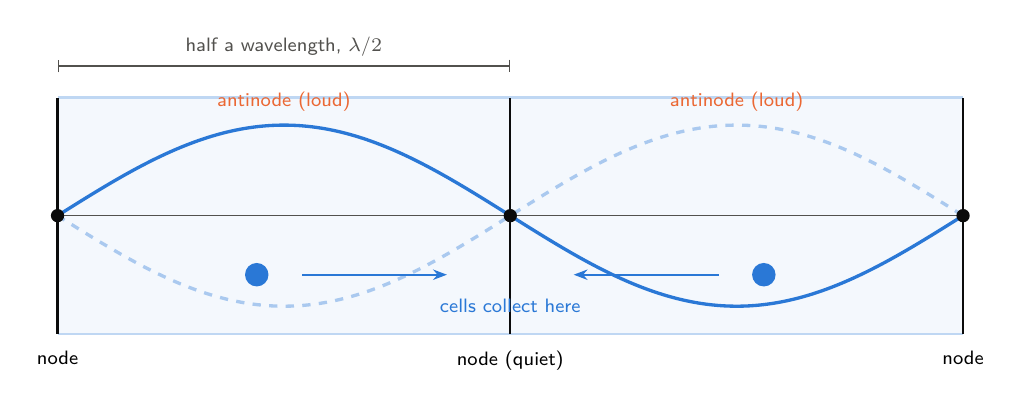
\begin{tikzpicture}[x=1.15cm,y=1cm]
  \fill[blue1!5] (0,-1.5) rectangle (10,1.5);
  \draw[blue1!30,thick] (0,-1.5) -- (10,-1.5);
  \draw[blue1!30,thick] (0,1.5) -- (10,1.5);
  % the standing wave envelope
  \draw[blue1,very thick,domain=0:10,samples=200] plot (\x,{1.15*sin(deg(pi*\x/5))});
  \draw[blue1!40,very thick,dashed,domain=0:10,samples=200]
        plot (\x,{-1.15*sin(deg(pi*\x/5))});
  \draw[muted,thin] (0,0) -- (10,0);
  % nodes
  \foreach \x in {0,5,10}{
    \draw[ink,thick] (\x,-1.5) -- (\x,1.5);
    \node[circle,fill=ink,inner sep=1.7pt] at (\x,0) {};
  }
  \node[below,font=\scriptsize\sffamily] at (0,-1.6) {node};
  \node[below,font=\scriptsize\sffamily] at (5,-1.6) {node (quiet)};
  \node[below,font=\scriptsize\sffamily] at (10,-1.6) {node};
  \node[above,font=\scriptsize\sffamily,orange1] at (2.5,1.2) {antinode (loud)};
  \node[above,font=\scriptsize\sffamily,orange1] at (7.5,1.2) {antinode (loud)};
  % cells drifting to the node
  \node[circle,fill=blue1,inner sep=3pt] (c1) at (2.2,-0.75) {};
  \node[circle,fill=blue1,inner sep=3pt] (c2) at (7.8,-0.75) {};
  \draw[-{Stealth[length=5pt]},blue1,thick] (2.7,-0.75) -- (4.3,-0.75);
  \draw[-{Stealth[length=5pt]},blue1,thick] (7.3,-0.75) -- (5.7,-0.75);
  \node[font=\scriptsize\sffamily,blue1] at (5,-1.15) {cells collect here};
  % scale bar
  \draw[|-|,muted] (0,1.9) -- (5,1.9)
      node[midway,above,font=\scriptsize\sffamily,color=muted] {half a wavelength, $\lambda/2$};
\end{tikzpicture}
\caption{A standing pressure wave across the channel. The solid and dashed
curves are the two extremes of the pressure swing. At the nodes the pressure
never changes; at the antinodes it swings hardest. Cells that are denser and
stiffer than water --- which is every cell in the body --- drift towards the
nodes.}
\end{figure}

The spacing between neighbouring nodes is always \emph{half} a wavelength. That
single fact is what lets us design the device: choose the wavelength, and you
have chosen where the cells will collect.

\section{Why a standing wave pushes things}

Here is the part that is genuinely surprising. The pressure at a node never
changes. So why would a cell sitting slightly off a node feel any push at all?

The answer is that the cell \emph{scatters} the sound. It is denser and stiffer
than the water around it, so it does not move quite in step with the liquid.
It re-radiates a small wave of its own, and that scattered wave interferes with
the original. When you average over one full cycle of the oscillation --- which
takes 150 nanoseconds, so ``averaged'' is a fair description of anything the
cell experiences --- the interference does not cancel. It leaves behind a small,
steady push.

\begin{analogy}
Imagine an invisible landscape of hills and valleys laid over the channel. A
cell placed on it rolls downhill, exactly like a marble. It is not being blown
along by the sound; it is sitting on a slope that the sound created.

The technical name for this landscape is the \textbf{Gor'kov potential}, after
the Soviet physicist who worked it out in 1962. Where the valleys are --- at
the quiet nodes or at the loud antinodes --- depends on the cell.
\end{analogy}

The height of this landscape at any point is:

\begin{equation}
U = V_c\left[\;\underbrace{\frac{f_1}{2}\,\kappa_f\,\langle p^2\rangle}_{\text{from squeezing}}
\;-\;\underbrace{\frac{3}{4}\,f_2\,\rho_f\,\langle v^2\rangle}_{\text{from sloshing}}\;\right]
\label{eq:gorkov}
\end{equation}

\begin{center}\small
\begin{tabular}{ll}
\sym{U}{the height of the landscape at that point \dims{joules}}
\sym{V_c}{the cell's volume, $\tfrac{4}{3}\pi r^3$ \dims{\si{\cubic\meter}}}
\sym{\langle p^2\rangle}{how hard the pressure swings there, averaged over a cycle}
\sym{\langle v^2\rangle}{how hard the water sloshes back and forth there, averaged}
\sym{\rho_f,\kappa_f}{the water's density and compressibility}
\sym{f_1,f_2}{two numbers describing how much the cell differs from water --- next section}
\end{tabular}
\end{center}

And the force is simply how steep the landscape is:

\begin{equation}
\boxed{\;F = -\nabla U\;}
\end{equation}

The $\nabla$ (``nabla'' or ``grad'') just means \emph{slope}. The minus sign
means downhill. That is the whole of it: build the landscape, measure its
slope, and you have the force.

\begin{plain}
The sound field creates an invisible hilly surface. Cells roll downhill on it.
The two terms in equation~\eqref{eq:gorkov} are the two reasons a cell is not
the same as the water it displaced: it resists being squeezed differently
(first term), and it resists being shaken differently (second term).
\end{plain}

\section{The contrast factor: two questions, one number}

The cell only has to answer two questions.

\begin{center}\small
\begin{tabular}{p{4.4cm}p{5.2cm}p{5.2cm}}
\toprule
\textbf{Question} & \textbf{The number} & \textbf{For a typical cell} \\
\midrule
Am I harder to squeeze than water? &
$f_1 = 1 - \dfrac{\kappa_p}{\kappa_f}$ (the \emph{monopole} term) &
$f_1 = 1 - \frac{3.72}{4.48} = 0.169$, so yes, a bit \\[10pt]
Am I heavier than water? &
$f_2 = \dfrac{2(\rho_p-\rho_f)}{2\rho_p+\rho_f}$ (the \emph{dipole} term) &
$f_2 = \frac{2(1068-997)}{2136+997} = 0.045$, so yes, slightly \\
\bottomrule
\end{tabular}
\end{center}

Combine them into a single \textbf{acoustic contrast factor}:

\begin{equation}
\Phi \;=\; f_1 + \tfrac{3}{2}f_2
\;=\; \frac{5\rho_p-2\rho_f}{2\rho_p+\rho_f}-\frac{\kappa_p}{\kappa_f}
\label{eq:phi}
\end{equation}

\begin{center}\small
\begin{tabular}{ll}
\sym{\Phi>0}{the cell is denser \emph{and} stiffer than water. It goes to the
\textbf{node}. Every cell in the human body does this.}
\sym{\Phi<0}{the cell is lighter or squishier. It goes to the \textbf{antinode}.
Fat droplets and gas bubbles do this.}
\sym{\Phi=0}{the object is acoustically indistinguishable from water, and nothing happens.}
\end{tabular}
\end{center}

\begin{center}\small
\begin{tabular}{lrl}
\toprule
\textbf{Particle} & $\Phi$ & \textbf{Where it goes} \\
\midrule
platelet & $+0.360$ & node \\
red blood cell & $+0.334$ & node \\
MCF-7 tumour cell & $+0.237$ & node \\
white blood cell & $+0.179$ & node \\
fat droplet & $-0.273$ & \textbf{antinode} \\
\bottomrule
\end{tabular}
\end{center}

The fat droplet is in the table on purpose: it is the test case. Any correct
implementation of equation~\eqref{eq:phi} \emph{must} return a negative number
for it, and the automated test suite checks exactly that.

\begin{warnbox}
\textbf{The three-times trap.} Two definitions of $\Phi$ circulate in the
published literature and they differ by a factor of exactly three. The one
above is the classical version. Some authors (including the most widely-cited
modern tutorial) use $\Phi_{\text{alt}} = f_1/3 + f_2/2 = \Phi/3$, together with
a force formula that has a compensating factor.

Mix them up and every force you compute is wrong by 3$\times$ --- and it will
look plausible, because it is still the right order of magnitude. The software
provides both under different names and the test suite pins their ratio at
exactly 3.
\end{warnbox}

\section{The one equation the whole device rests on}

For a one-dimensional standing wave, doing the slope calculation on
equation~\eqref{eq:gorkov} gives:

\begin{keybox}
\begin{equation}
F_r(x) \;=\; -\,\frac{\pi\, p_0^{\,2}\, V_c\, \kappa_f}{2\lambda}\;\Phi\;
\sin\!\big(2k(x-x_{\text{node}})\big)
\label{eq:force}
\end{equation}
\vspace{-4pt}
\begin{center}\small
\begin{tabular}{ll}
\sym{F_r}{the sideways push on the cell \dims{newtons}}
\sym{x}{where the cell is, measured across the channel}
\sym{x_{\text{node}}}{where the nearest quiet spot is}
\sym{p_0}{how loud the sound is (pressure amplitude) \dims{pascals}}
\sym{V_c}{the cell's volume $=\tfrac43\pi r^3$}
\sym{\kappa_f}{how squeezable water is}
\sym{\lambda}{the wavelength of the standing pattern}
\sym{k}{$=2\pi/\lambda$, just wavelength written the way physicists prefer}
\sym{\Phi}{the contrast factor from equation~\eqref{eq:phi}}
\end{tabular}
\end{center}
\end{keybox}

Read it one piece at a time.

\begin{itemize}
\item \textbf{$\sin(2k(x-x_{\text{node}}))$} --- the direction. It is zero
exactly at the node and exactly at the antinode, positive on one side and
negative on the other. So the cell is always pushed towards the node, and once
it arrives, the force switches off. It parks there.
\item \textbf{$p_0^2$} --- turn the sound up twice as loud and the push
quadruples. Not doubles. This is why the drive voltage is such an effective
knob.
\item \textbf{$V_c \propto r^3$} --- \emph{this is the whole device}, and it
gets its own section.
\item \textbf{$\Phi$} --- which way and how strongly the cell responds.
\item \textbf{$1/\lambda$} --- a tighter pattern pushes harder, because the
landscape has steeper slopes.
\end{itemize}

\section{Why size wins: the $r^2$ law}
\label{sec:r2}

The cell is not in a vacuum. It is in water, and water resists. The resistance
is \textbf{Stokes drag}:

\begin{equation}
F_d = 6\pi\mu r\,(u_f - u_p)
\label{eq:stokes}
\end{equation}

\begin{center}\small
\begin{tabular}{ll}
\sym{\mu}{how thick the liquid is (viscosity); water is
\SI{0.89e-3}{\pascal\second}}
\sym{r}{the cell's radius --- note: \textbf{radius}, not volume}
\sym{u_f-u_p}{how fast the cell is moving relative to the water around it}
\end{tabular}
\end{center}

Now put the two together. The cell speeds up until the push and the drag
balance, which happens almost instantly (see \S\ref{sec:lowre}). At balance:

\begin{equation}
\underbrace{\;\text{push} \;\propto\; r^3\;}_{\text{equation \eqref{eq:force}}}
\;=\;
\underbrace{\;\text{drag} \;\propto\; r \times \text{speed}\;}_{\text{equation \eqref{eq:stokes}}}
\qquad\Longrightarrow\qquad
\boxed{\ \text{speed} \;\propto\; r^2\ }
\end{equation}

\begin{plain}
The push grows with the cell's \emph{volume}. The resistance grows only with its
\emph{radius}. Volume beats radius. Double the radius and the cell moves four
times faster.
\end{plain}

\begin{analogy}
Drop a marble and a cannonball into a swimming pool. Both feel gravity pulling
on their whole volume and water resisting only across their width. The
cannonball wins, and not by a little. Acoustic sorting is exactly this, with
sound instead of gravity, sideways instead of down.
\end{analogy}

Put the real numbers in. Comparing an MCF-7 tumour cell to a red blood cell:

\begin{align}
\frac{\text{speed of MCF-7}}{\text{speed of RBC}}
&= \left(\frac{r_{\text{MCF-7}}}{r_{\text{RBC}}}\right)^{\!2}
   \times \frac{\Phi_{\text{MCF-7}}}{\Phi_{\text{RBC}}} \notag\\[4pt]
&= \left(\frac{9.00}{2.78}\right)^{\!2} \times \frac{0.179}{0.252}
 \;=\; 10.5 \times 0.71 \;=\; \mathbf{7.4}
\end{align}

The tumour cell crosses the channel 7.4 times faster than the red cell. Give
them both the same amount of time --- which is what a fixed channel length
does --- and the tumour cell arrives at the middle while the red cell is still
most of the way out.

\begin{figure}[h]
\centering
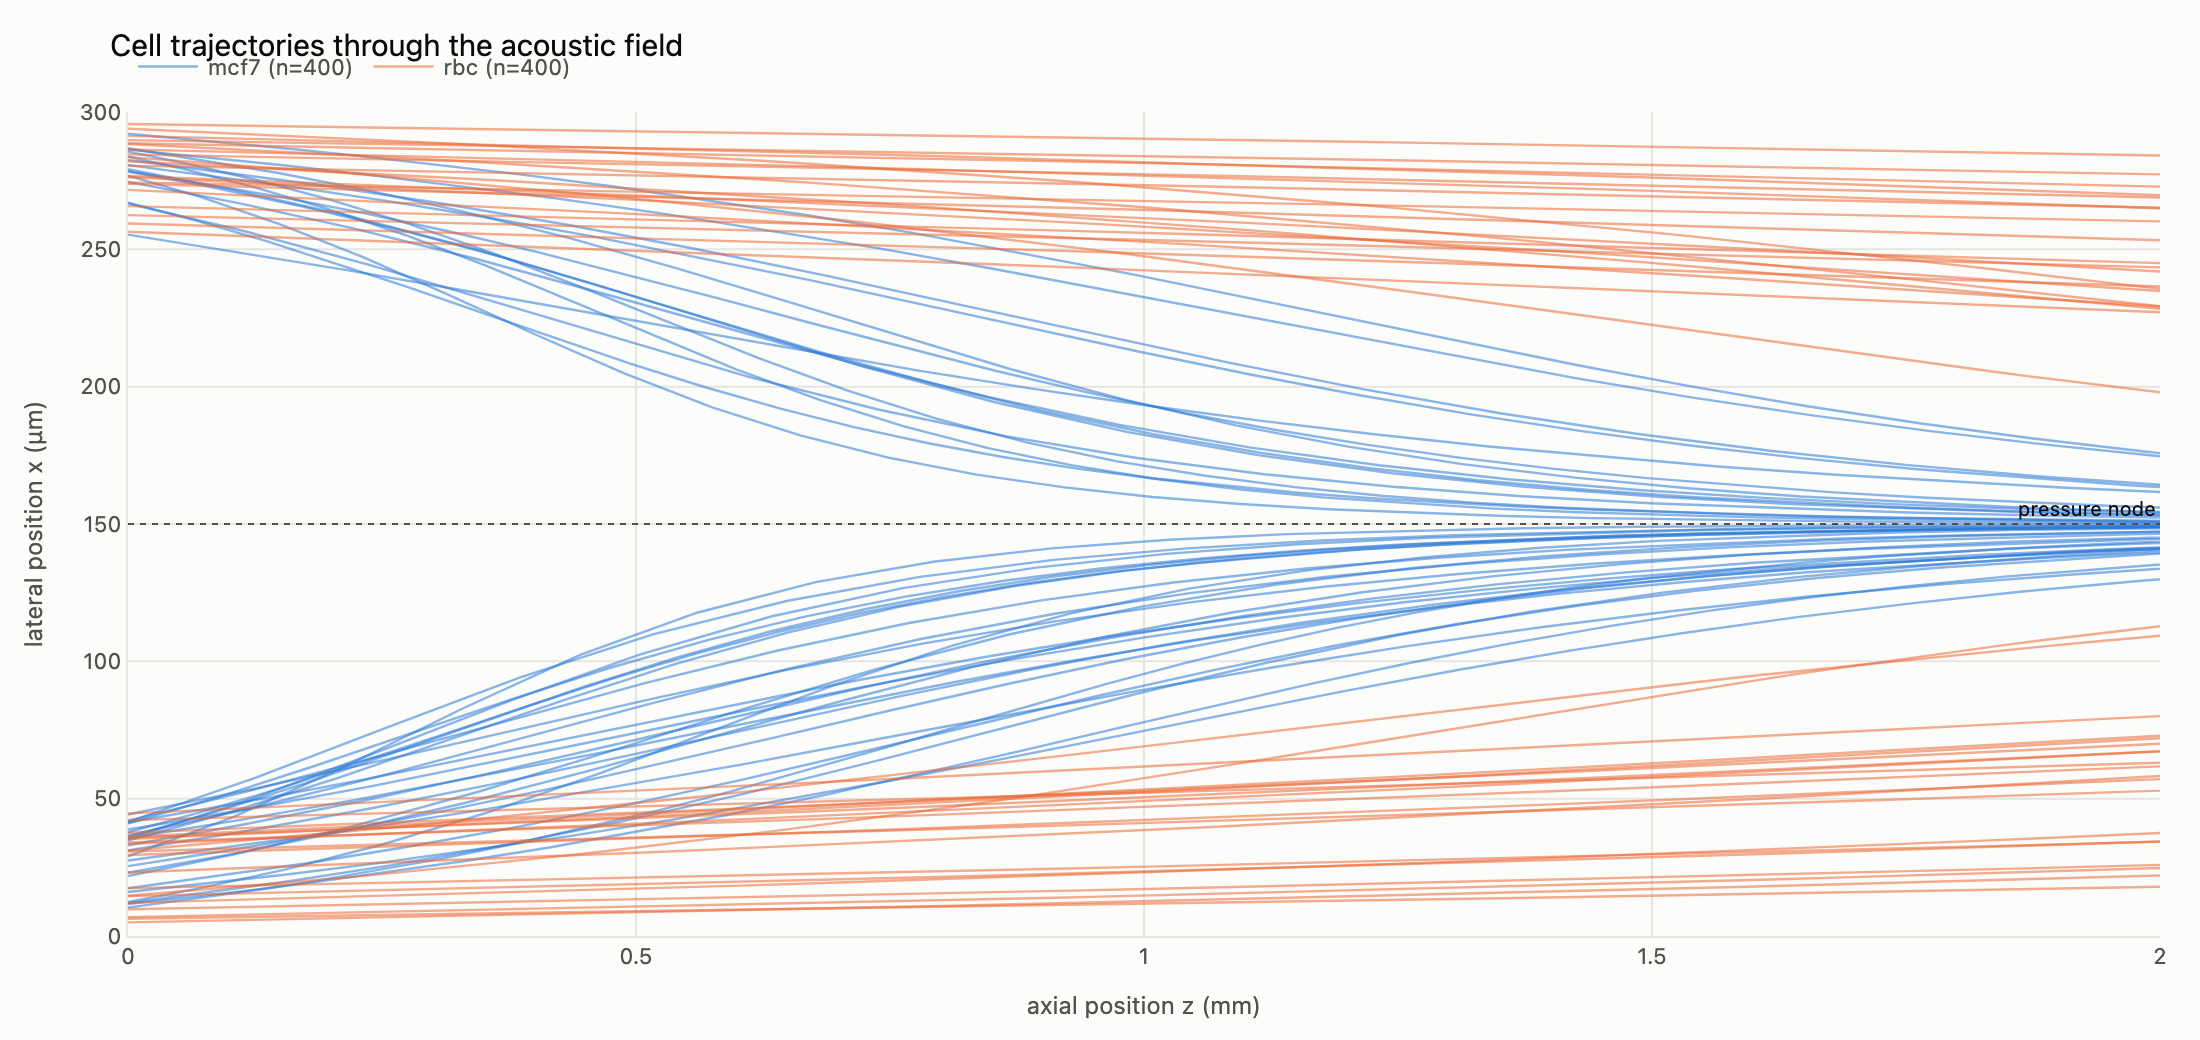
\includegraphics[width=0.94\textwidth]{../../assets/02_trajectories.png}
\caption{The $r^2$ law, simulated. 400 tumour cells (blue) and 400 red blood
cells (orange) enter at the two walls and travel \SI{2}{\milli\meter} down the
channel, which takes \SI{0.36}{\second}. The tumour cells reach the middle; the
red cells barely move. Nothing else is going on in this device.}
\end{figure}

Note that the contrast factor actually works \emph{against} us --- the red cell
has a higher $\Phi$ (0.252 vs 0.179), because it is denser and stiffer relative
to water than a tumour cell is. Size overwhelms it anyway, ten to one.

\section{Where the sound comes from: an earthquake on a chip}

We need a standing sound wave inside a channel \SI{300}{\micro\meter} wide.
There is no room for a loudspeaker. Instead, the channel sits on top of a slab
of \textbf{lithium niobate}, a crystal that is \emph{piezoelectric}: apply a
voltage and it physically deforms; deform it and it produces a voltage.

On the surface of that crystal we lay down two interlocking metal combs, called
an \textbf{interdigital transducer} or IDT. Apply an alternating voltage across
the combs, and the crystal ripples --- a tiny, extremely fast earthquake
confined to the top surface. This is a \textbf{surface acoustic wave}.

\begin{figure}[h]
\centering
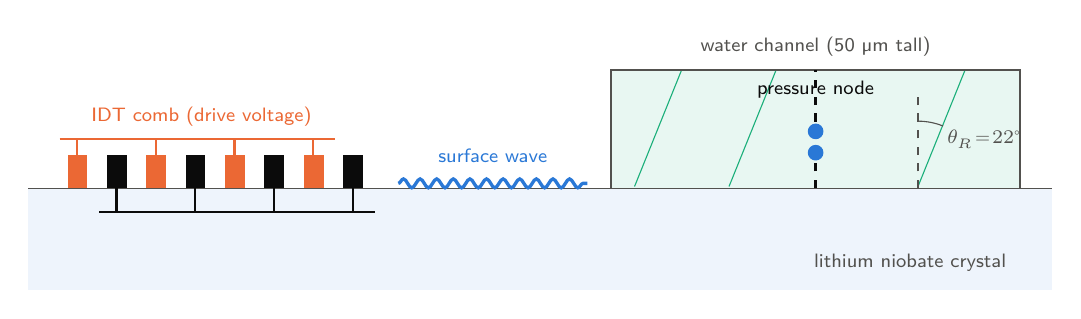
\begin{tikzpicture}[x=1cm,y=1cm]
  % substrate
  \fill[blue1!8] (0,-1.3) rectangle (13,0);
  \draw[muted] (0,0) -- (13,0);
  \node[font=\scriptsize\sffamily,color=muted] at (11.2,-0.95)
        {lithium niobate crystal};
  % IDT fingers
  \foreach \x in {0.5,1.5,2.5,3.5}{
    \fill[orange1] (\x,0) rectangle (\x+0.25,0.42);}
  \foreach \x in {1.0,2.0,3.0,4.0}{
    \fill[ink] (\x,0) rectangle (\x+0.25,0.42);}
  \draw[orange1,thick] (0.4,0.62) -- (3.9,0.62);
  \foreach \x in {0.5,1.5,2.5,3.5}{\draw[orange1,thick] (\x+0.12,0.42)--(\x+0.12,0.62);}
  \draw[ink,thick] (0.9,-0.3) -- (4.4,-0.3);
  \foreach \x in {1.0,2.0,3.0,4.0}{\draw[ink,thick] (\x+0.12,0)--(\x+0.12,-0.3);}
  \node[font=\scriptsize\sffamily,color=orange1,above] at (2.2,0.66)
       {IDT comb (drive voltage)};
  % surface wave ripple
  \draw[blue1,very thick,decorate,
        decoration={snake,amplitude=1.6pt,segment length=6pt}] (4.7,0.06) -- (7.1,0.06);
  \node[font=\scriptsize\sffamily,color=blue1,above] at (5.9,0.2) {surface wave};
  % channel
  \fill[aqua1!10] (7.4,0) rectangle (12.6,1.5);
  \node[font=\scriptsize\sffamily,color=muted,above] at (10,1.55)
       {water channel (50 µm tall)};
  % leaking rays: theta_R is measured FROM THE VERTICAL, so 90-22 = 68 deg
  \begin{scope}
    \clip (7.4,0) rectangle (12.6,1.5);
    \foreach \x in {7.7,8.9,11.3}{
      \draw[-{Stealth[length=4pt]},aqua1] (\x,0.02) -- ++(68:1.9);}
  \end{scope}
  \draw[muted,thick] (7.4,0) -- (7.4,1.5) -- (12.6,1.5) -- (12.6,0);
  % angle annotation, in a clear part of the channel
  \draw[muted,dashed] (11.3,0) -- (11.3,1.25);
  \draw[muted] (11.3,0.85) arc (90:68:0.85);
  \node[font=\scriptsize,color=muted,right] at (11.55,0.62) {$\theta_R\!=\!22^\circ$};
  % pressure node line
  \draw[ink,very thick,dashed] (10,0) -- (10,1.5);
  \node[font=\scriptsize\sffamily,color=ink,above] at (10,1.02)
       {\,pressure node\,};
  \node[circle,fill=blue1,inner sep=2pt] at (10,0.45) {};
  \node[circle,fill=blue1,inner sep=2pt] at (10,0.72) {};
\end{tikzpicture}
\caption{The device in cross-section. A comb-shaped electrode drives a ripple
along the crystal surface. Because the ripple travels faster in the crystal
(\SI{3979}{\meter\per\second}) than sound does in water
(\SI{1497}{\meter\per\second}), it leaks into the liquid at a fixed angle of
about $22^\circ$ --- the same reason a straw looks bent in a glass of water.
Two such waves sent from opposite sides make the standing pattern.}
\end{figure}

The leak angle is set by the same rule that bends light entering water:

\begin{equation}
\theta_R = \arcsin\!\left(\frac{c_{\text{water}}}{c_{\text{SAW}}}\right)
= \arcsin\!\left(\frac{1497}{3979}\right) = 22.1^\circ
\end{equation}

We do not put this angle into the simulation. We tell the computer what the
crystal surface is doing, ask it to solve the equation for sound in water, and
the $22^\circ$ comes out on its own. That is a small but real check that the
physics is being solved rather than assumed.

% ============================================================================
\clearpage
\section{Two things the textbook formula gets wrong here}

Building this software turned up two places where applying the standard
equations naively gives the wrong answer. Both are now handled explicitly, and
both are the sort of thing that would quietly ruin a device design.

\subsection{The ruler is the crystal, not the water}
\label{sec:ruler}

The obvious thing to assume is that the sound in the channel has the wavelength
of sound in water: $\lambda_{\text{water}} = c_{\text{water}}/f$. At
\SI{20}{\mega\hertz} that is \SI{75}{\micro\meter}, so nodes every
\SI{37}{\micro\meter}.

That is wrong. The pattern in the liquid is stamped onto it by the crystal
underneath, so it inherits the crystal's spacing, not the water's:

\begin{equation}
\lambda_{\text{SAW}} = \frac{c_{\text{SAW}}}{f},
\qquad
\text{node spacing} = \frac{\lambda_{\text{SAW}}}{2}
\end{equation}

At \SI{20}{\mega\hertz}, $\lambda_{\text{SAW}} = 3979/20\times10^{6} =
\SI{199}{\micro\meter}$, so nodes every \SI{99.5}{\micro\meter} --- nearly three
times further apart than the naive answer.

\begin{center}\small
\begin{tabular}{rrrr}
\toprule
\textbf{Frequency} & \textbf{$\lambda_{\text{SAW}}$} & \textbf{Node spacing} &
\textbf{Nodes in a \SI{300}{\micro\meter} channel} \\
\midrule
\SI{6.632}{\mega\hertz} & \SI{600}{\micro\meter} & \SI{300}{\micro\meter} & \textbf{1} \\
\SI{13.26}{\mega\hertz} & \SI{300}{\micro\meter} & \SI{150}{\micro\meter} & 2 \\
\SI{20}{\mega\hertz}    & \SI{199}{\micro\meter} & \SI{99.5}{\micro\meter} & 3 \\
\bottomrule
\end{tabular}
\end{center}

\begin{warnbox}
This is not a detail. A sorter with \textbf{one} node in the channel collects
everything into the middle and you tap the middle outlet. A sorter with
\textbf{three} nodes collects cells into three separate stripes, each cell going
to whichever stripe it started nearest. The outlet histogram becomes
three-humped and the two-outlet design simply does not work.

The original specification for this project asked for \SI{20}{\mega\hertz} in a
\SI{300}{\micro\meter} channel. That combination has three nodes. The software
now detects this and prints the frequency that gives one:
\[
f = \frac{c_{\text{SAW}}}{2W} = \frac{3979}{2\times300\times10^{-6}}
  = \SI{6.632}{\mega\hertz}
\]
which is the default in the shipped configuration.
\end{warnbox}

\subsection{The sound does not travel straight across}

The second correction is subtler. The standard force formula, equation
\eqref{eq:force}, quietly assumes the wave travels purely \emph{across} the
channel. In this device it does not: the crystal sets the sideways spacing, and
the laws of sound in water then force the wave to have an upward component as
well. That upward component is precisely the $22^\circ$ leak.

Writing $k_x$ for the sideways wavenumber (set by the crystal) and $k_f$ for
what sound in water would have, they are related by Pythagoras:

\begin{equation}
k_x^2 + k_y^2 = k_f^2,
\qquad k_x = \frac{2\pi}{\lambda_{\text{SAW}}},
\qquad k_f = \frac{2\pi f}{c_{\text{water}}}
\end{equation}

Redoing the Gor'kov calculation with the tilt included gives a modified contrast
factor:

\begin{equation}
\boxed{\;\Phi_{\text{eff}} = f_1 + \tfrac{3}{2}f_2\left(\frac{k_x}{k_f}\right)^{\!2}\;}
\label{eq:phieff}
\end{equation}

The squeezing term is untouched; the sloshing term is scaled down, because the
water is sloshing partly up-and-down rather than side-to-side, and only the
side-to-side part contributes to sideways force. When $k_x = k_f$ --- a wave
that really does travel straight across --- the correction disappears and the
textbook formula returns exactly.

\begin{center}\small
\begin{tabular}{lrrr}
\toprule
\textbf{Cell} & $\Phi$ \textbf{(textbook)} & $\Phi_{\text{eff}}$ \textbf{(this device)} & \textbf{Change} \\
\midrule
MCF-7 & 0.2371 & 0.1787 & $-25\,\%$ \\
red blood cell & 0.3341 & 0.2519 & $-25\,\%$ \\
\bottomrule
\end{tabular}
\end{center}

A 25\,\% error in force is a 25\,\% error in how far every cell travels, which
near the edge of a collection outlet is the difference between a working device
and a broken one. The correction is verified in the test suite by computing the
force numerically from an exact solution of the wave equation and comparing:
they agree to seven parts in a million.

\section{Life at low Reynolds number: water is honey}
\label{sec:lowre}

At the scale of a cell, water does not behave the way your intuition says.
The governing quantity is the \textbf{Reynolds number}, a pure ratio with no
units:

\begin{equation}
\mathrm{Re} = \frac{\rho\, U\, L}{\mu}
= \frac{\text{how much the fluid wants to keep going}}{\text{how much it wants to stop}}
\end{equation}

\begin{center}\small
\begin{tabular}{lr>{\raggedright\arraybackslash}p{7.4cm}}
\toprule
\textbf{Situation} & $\mathrm{Re}$ & \textbf{What it feels like} \\
\midrule
A person swimming & $10^{6}$ & you glide when you stop stroking \\
A goldfish & $10^{4}$ & still glides \\
\textbf{Our channel} & $\mathbf{0.53}$ & no gliding at all \\
\textbf{A cell in our channel} & $\mathbf{0.15}$ & --- \\
A bacterium swimming & $10^{-5}$ & like swimming in tar \\
\bottomrule
\end{tabular}
\end{center}

\begin{analogy}
Stop pushing a cell and it does not coast. It stops within about
\SI{50}{\nano\meter} --- less than one hundredth of its own diameter --- in
about \SI{20}{\micro\second}. There is no momentum, no drifting, no
overshoot. The cell's velocity is determined entirely by the forces acting on
it \emph{right now}.
\end{analogy}

This is enormously convenient. Newton's second law, $F = ma$, is a differential
equation in acceleration and needs two starting conditions. But when there is no
meaningful acceleration, it collapses to something you can almost do in your
head:

\begin{equation}
\underbrace{v}_{\text{cell speed}}
= \underbrace{u_f}_{\text{speed of the water}}
+ \underbrace{\frac{F}{6\pi\mu r}}_{\text{extra speed from the push}}
\label{eq:overdamped}
\end{equation}

The simulation uses this by default. It also implements the full
$F=ma$ version, and the test suite checks that the two agree --- which is how
we know the approximation is safe here rather than merely convenient.

\begin{warnbox}
This breaks if the flow is fast enough or the particles large enough that
$\mathrm{Re}$ approaches 1. The software computes both Reynolds numbers on every
single run and prints a warning if either exceeds 1, rather than silently
producing a number that looks fine and is wrong.
\end{warnbox}

\section{How the liquid flows: the parabola}

The cells are carried along the channel by liquid pushed from a syringe pump.
That flow is not uniform: it sticks to the walls (the ``no-slip'' condition,
which is why blowing on a dusty surface never quite cleans it) and moves fastest
in the middle.

\begin{figure}[h]
\centering
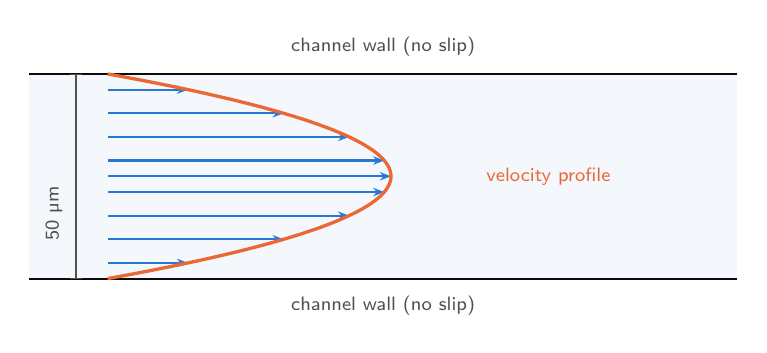
\begin{tikzpicture}[x=1cm,y=1cm]
  \fill[blue1!5] (0,0) rectangle (9,2.6);
  \draw[ink,thick] (0,0)--(9,0);
  \draw[ink,thick] (0,2.6)--(9,2.6);
  \node[font=\scriptsize\sffamily,color=muted,below] at (4.5,-0.1) {channel wall (no slip)};
  \node[font=\scriptsize\sffamily,color=muted,above] at (4.5,2.7) {channel wall (no slip)};
  \foreach \y in {0.2,0.5,0.8,1.1,1.3,1.5,1.8,2.1,2.4}{
    \pgfmathsetmacro\L{3.6*(1-((\y-1.3)/1.3)^2)}
    \draw[-{Stealth[length=4pt]},blue1,thick] (1,\y) -- (1+\L,\y);
  }
  \draw[orange1,very thick,domain=0:2.6,samples=60,smooth]
        plot ({1+3.6*(1-((\x-1.3)/1.3)^2)},\x);
  \node[font=\scriptsize\sffamily,color=orange1] at (6.6,1.3)
       {velocity profile};
  \draw[|-|,muted] (0.6,0)--(0.6,2.6)
       node[midway,left,font=\scriptsize\sffamily,color=muted,rotate=90,yshift=8pt] {50 µm};
\end{tikzpicture}
\caption{Pressure-driven flow in a channel. Zero at the walls, fastest in the
middle. A cell near a wall takes much longer to travel the channel than one in
the middle --- which is why the simulation has to integrate long enough for the
slowest cell, not the average one.}
\end{figure}

For a rectangular channel there is an exact answer, written as an infinite sum:

\begin{equation}
u_z(x,y)=\frac{16 b^2 G}{\mu\pi^3}\sum_{n=1,3,5,\dots}
\frac{(-1)^{(n-1)/2}}{n^3}
\left[1-\frac{\cosh\!\big(\tfrac{n\pi x}{2b}\big)}{\cosh\!\big(\tfrac{n\pi a}{2b}\big)}\right]
\cos\!\left(\frac{n\pi y}{2b}\right)
\end{equation}

\begin{center}\small
\begin{tabular}{ll}
\sym{u_z}{how fast the liquid moves along the channel at the point $(x,y)$}
\sym{a,b}{half the channel's width and height}
\sym{G}{the pressure drop per metre pushing the liquid along}
\sym{n}{the sum index; each term is a smaller correction than the last}
\end{tabular}
\end{center}

\begin{plain}
This looks alarming and is not. It is a recipe: add up a few wavy shapes with
decreasing weights and you get the parabola-like profile in the figure. Thirty
terms are enough for six-digit accuracy. The software uses the exact sum rather
than solving the flow numerically, because the exact answer is both faster and
more accurate.
\end{plain}

For the standard operating point --- \SI{5}{\micro\liter\per\minute} through a
\SI{300}{}$\times$\SI{50}{\micro\meter} channel --- this gives:

\begin{center}\small
\begin{tabular}{lr}
\toprule
average speed & \SI{5.56}{\milli\meter\per\second} \\
peak speed (centre) & \SI{9.31}{\milli\meter\per\second} \\
time to cross the \SI{2}{\milli\meter} active region & \SI{0.36}{\second} \\
pressure needed & \SI{26.5}{\kilo\pascal\per\meter} \\
\bottomrule
\end{tabular}
\end{center}

\textbf{That \SI{0.36}{\second} is the entire budget.} Every cell you want to
collect has to reach the middle of the channel in 0.36 seconds, and every cell
you want to discard has to fail to. Everything in the design --- the frequency,
the voltage, the flow rate, the length --- is in service of that one race.

% ============================================================================
\clearpage
\part*{Part III --- The second instrument: counting cells with electricity}
\addcontentsline{toc}{part}{Part III --- Counting cells with electricity}

\section{A cell is a tiny insulator}

The sorter answers ``which cells are these?''. A different question a laboratory
asks constantly is ``how many cells are there, and are they still alive?'' ---
for example, every hour for two days while testing whether a drug kills them.

Photographing the dish every hour and counting by eye is slow and disturbs the
cells. There is a much better trick, and it relies on a fact about cell
membranes:

\begin{plain}
The membrane around a cell is a double layer of fat molecules about
\SI{5}{\nano\meter} thick. Fat does not conduct electricity. So a cell is, to a
first approximation, a bag of salt water --- which conducts well --- wrapped in
an insulating skin.
\end{plain}

Put gold electrodes in the bottom of the dish and pass a tiny alternating
current. When the dish is empty, the current flows freely through the salty
growth medium. As cells settle and spread on the electrodes, they get in the
way: the current has to squeeze through the narrow gaps between the cells and
through the even narrower gap underneath them.

\begin{analogy}
It is like laying cling film over a wire mesh at the bottom of a stream. The
water has to find its way around the edges. The more cling film, the more the
flow is obstructed --- and the obstruction is something you can measure from
outside without touching the water.
\end{analogy}

More cells $\Rightarrow$ more obstruction $\Rightarrow$ higher \textbf{impedance}.
Impedance is just electrical resistance for alternating current, with one extra
feature: it has a size \emph{and} a timing shift, so it is written as a complex
number $Z$.

\begin{figure}[h]
\centering
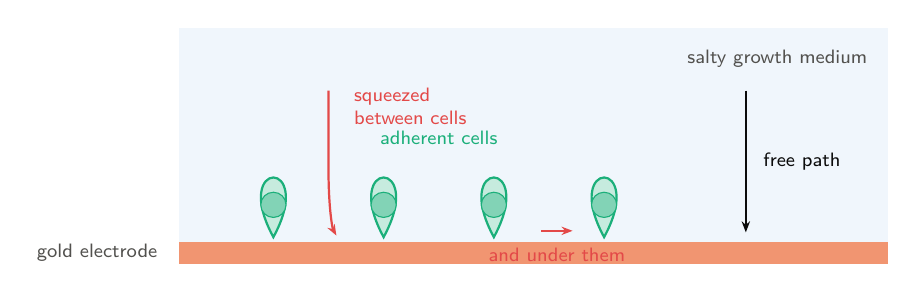
\begin{tikzpicture}[x=1cm,y=1cm,font=\scriptsize\sffamily]
  % electrode
  \fill[orange1!70] (0,0) rectangle (9,0.28);
  \node[left,color=muted] at (-0.15,0.14) {gold electrode};
  % medium
  \fill[blue1!7] (0,0.28) rectangle (9,3);
  \node[color=muted] at (7.6,2.6) {salty growth medium};
  % cells
  \foreach \x in {1.2,2.6,4.0,5.4}{
    \draw[fill=aqua1!25,draw=aqua1,thick]
      (\x,0.34) .. controls (\x-0.55,1.35) and (\x+0.55,1.35) .. (\x,0.34) -- cycle;
    \draw[fill=aqua1!55,draw=aqua1] (\x,0.75) circle (0.16);
  }
  \node[color=aqua1] at (3.3,1.6) {adherent cells};
  % current paths
  \draw[-{Stealth[length=4pt]},ink,thick] (7.2,2.2) -- (7.2,0.4);
  \node[right,color=ink] at (7.3,1.3) {free path};
  \draw[-{Stealth[length=4pt]},red1,thick]
       (1.9,2.2) -- (1.9,1.2) .. controls (1.9,0.7) and (1.95,0.45) .. (2.0,0.36);
  \node[right,color=red1,align=left] at (2.1,2.0) {squeezed\\between cells};
  \draw[-{Stealth[length=4pt]},red1,thick] (4.6,0.42) -- (5.0,0.42);
  \node[below,color=red1] at (4.8,0.32) {and under them};
\end{tikzpicture}
\caption{Electric cell-substrate impedance sensing. Current takes the easy route
where the electrode is bare and has to squeeze through gaps where cells sit. The
measured impedance therefore reports how much of the electrode is covered.}
\end{figure}

\section{Turning impedance into a growth curve}

The full relationship between how covered the electrode is and what the meter
reads was worked out by Giaever and Keese in 1991. It is not pretty:

\begin{equation}
\frac{1}{Z_c}=\frac{1}{Z_n}\left[
\frac{Z_n}{Z_n+Z_m}+\frac{Z_m/(Z_n+Z_m)}
{\dfrac{\gamma I_0(\gamma)}{2 I_1(\gamma)}+R_b\!\left(\dfrac{1}{Z_n}+\dfrac{1}{Z_m}\right)}\right],
\qquad
\gamma=\alpha\sqrt{\frac{1}{Z_n}+\frac{1}{Z_m}}
\end{equation}

\begin{center}\small
\begin{tabular}{ll}
\sym{Z_c}{what you measure when cells are present}
\sym{Z_n}{what you measure when the electrode is bare}
\sym{Z_m}{the resistance of the cell membranes themselves}
\sym{R_b}{how tightly the cells are sealed to each other --- ``tight junctions''}
\sym{\alpha}{how narrow the gap is between the cell's underside and the gold}
\sym{I_0,I_1}{Bessel functions --- standard mathematical functions that appear
whenever something spreads out radially from a point, which is what the current
under a round cell does}
\end{tabular}
\end{center}

\begin{plain}
Do not read the formula. Read what goes into it: how bare is the electrode, how
insulating are the membranes, how tightly are the cells stuck to each other, and
how thin is the gap underneath them. Those four things determine the reading.
The equation is just the bookkeeping.
\end{plain}

Laboratory instruments report a simplified, unitless version called the
\textbf{Cell Index}:

\begin{equation}
\mathrm{CI}(t)=\frac{|Z_{\text{cells}}(t)|-|Z_{\text{background}}|}{Z_{\text{reference}}}
\end{equation}

Zero means an empty electrode. It climbs as the cells attach, spread and divide.
It falls when they die and round up.

\begin{figure}[h]
\centering
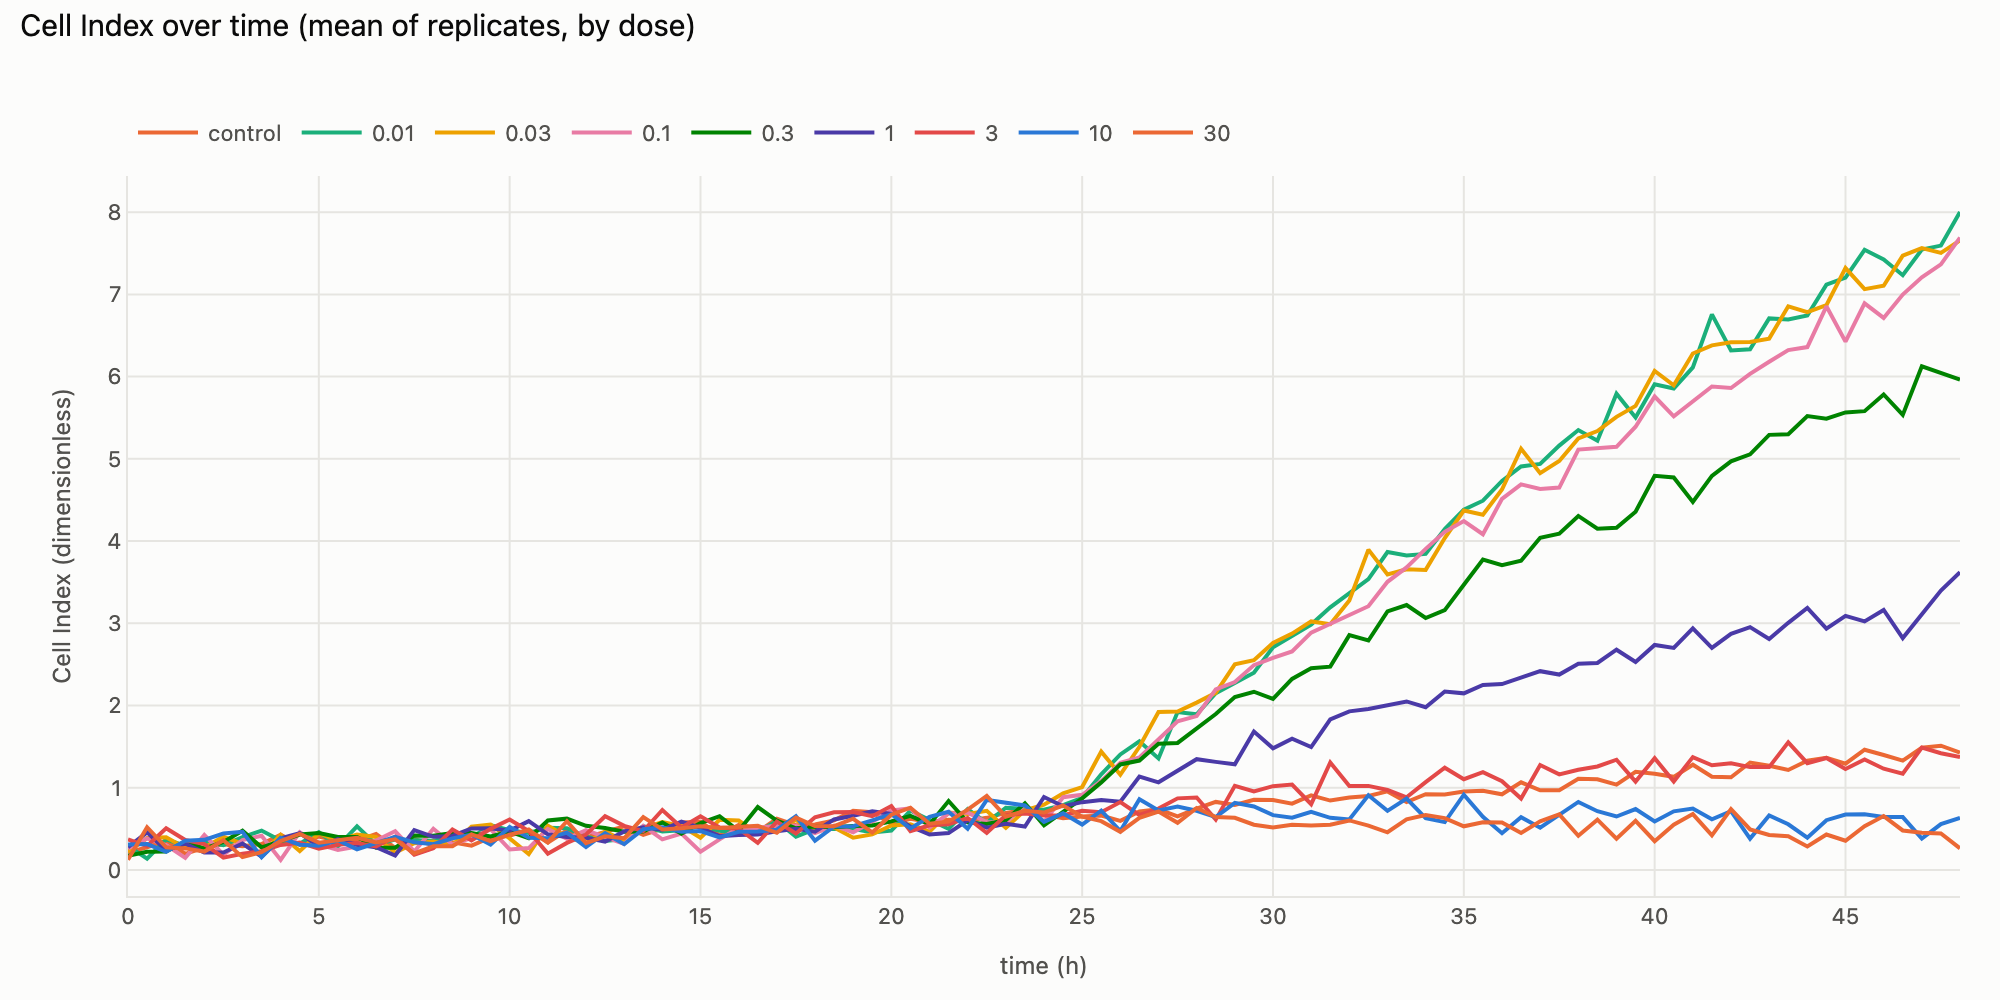
\includegraphics[width=0.86\textwidth]{../../assets/05_cell_index.png}
\caption{Simulated Cell Index over 48 hours, one line per drug dose. All wells
grow identically for the first 24 hours; the drug is added at hour 24 and the
curves separate by dose. This is the raw output of a real instrument, and this
plot is what the simulation reproduces.}
\end{figure}

\section{IC50: the number a drug is judged by}

Take the Cell Index at the end of the experiment, plot it against drug
concentration, and you get an S-shaped curve on a logarithmic axis: no effect at
low dose, everything dead at high dose, and a transition in between. Fit it with
the standard four-parameter logistic:

\begin{equation}
y=y_{\min}+\frac{y_{\max}-y_{\min}}{1+\left(c/\mathrm{IC}_{50}\right)^{h}}
\end{equation}

\begin{center}\small
\begin{tabular}{ll}
\sym{c}{drug concentration}
\sym{y}{how much cell signal is left}
\sym{\mathrm{IC}_{50}}{\textbf{the answer}: the concentration that kills half of them}
\sym{h}{the Hill slope --- how sharp the switch from ``alive'' to ``dead'' is}
\end{tabular}
\end{center}

\begin{figure}[h]
\centering
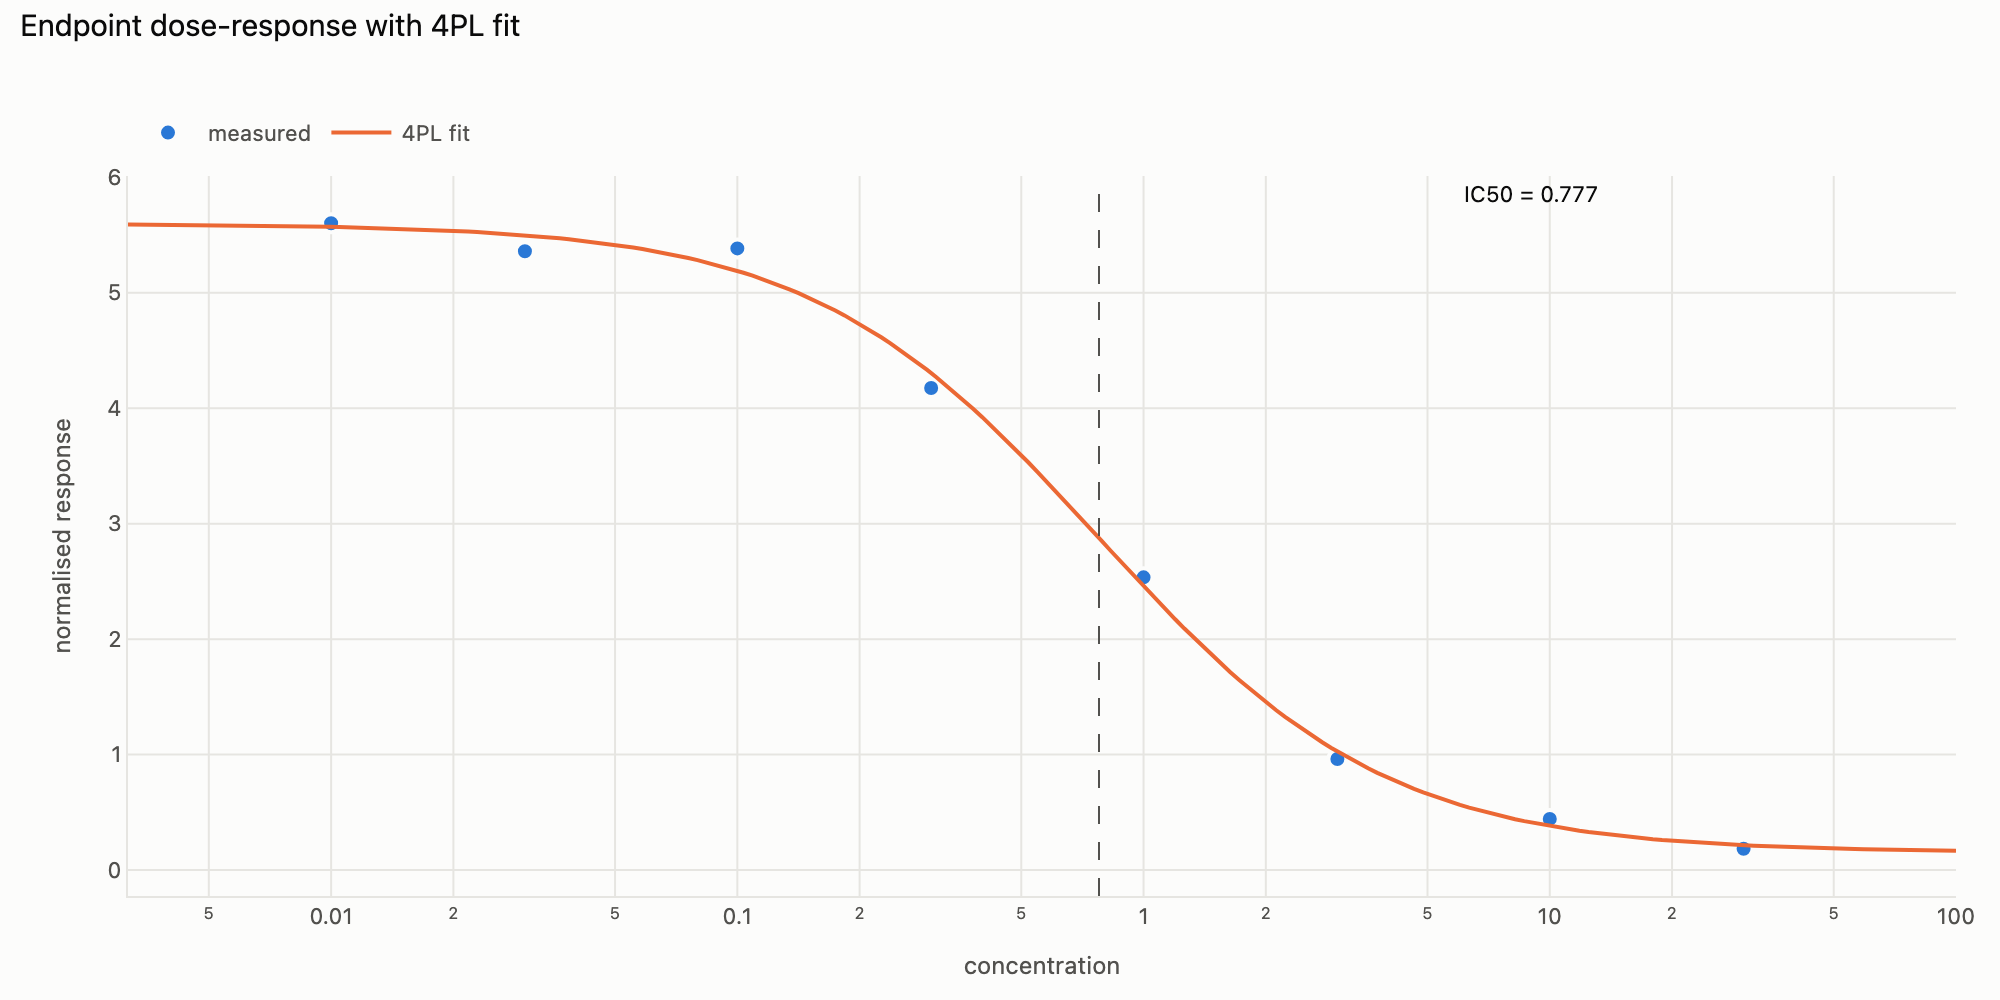
\includegraphics[width=0.78\textwidth]{../../assets/05_dose_response.png}
\caption{Dose--response from the simulated plate, with the fitted curve and the
extracted IC50.}
\end{figure}

\begin{warnbox}
\textbf{An honest wrinkle the simulation reproduces.} If you plant a true IC50
of 1.0 in the simulation and then measure it from the endpoint, you get 0.75.
That is not a bug.

The drug acts for 24 hours against cells that take about 20 hours to double, so
the population has not finished responding when you stop the experiment. The
measured IC50 always drifts towards its true value as exposure lengthens. Real
endpoint assays do exactly this, which is why published IC50 values are
meaningless without the exposure time attached.
\end{warnbox}

% ============================================================================
\clearpage
\part*{Part IV --- The third and fourth instruments: looking at pictures}
\addcontentsline{toc}{part}{Part IV --- Looking at pictures}

\section{Finding cells in an image}

Given a photograph down a microscope, how does a computer count the cells?

The naive answer --- ``anything brighter than a threshold is a cell'' ---
fails on real images for three reasons, and each step of the pipeline exists to
undo one of them:

\begin{center}\small
\begin{tabular}{p{4.6cm}p{5.0cm}p{5.0cm}}
\toprule
\textbf{Problem} & \textbf{Why it happens} & \textbf{The fix} \\
\midrule
The image is brighter in the middle than the corners &
the lamp is not perfectly even &
subtract a heavily blurred copy of the image from itself \\[4pt]
The image is speckly &
light arrives as discrete photons, and counting anything random has
$\sqrt{N}$ noise &
blur slightly \\[4pt]
Touching cells merge into one blob &
they are genuinely touching &
watershed, below \\
\bottomrule
\end{tabular}
\end{center}

\begin{analogy}
\textbf{Watershed.} Read the image as a landscape where bright means high, then
turn it upside down so each cell becomes a basin. Now flood the whole terrain
from the bottom of every basin at once. Where two floods meet, build a wall.
Those walls are the boundaries between touching cells.

The name is literal: it is the same computation a geographer does to work out
which river a raindrop will end up in.
\end{analogy}

The software also generates its own test images, with the true answer known
exactly, so the pipeline can be \emph{scored} rather than admired. On a
synthetic field of 150 cells it recovers 126. The 24 it misses are cells
touching the frame edge (deliberately discarded --- a cell cut in half by the
edge has no measurable size) and a few genuinely merged pairs.

\section{Counting, and why 100 cells means $\pm10\,\%$}

Once cells are found, concentration is geometry. A standard counting chamber
has a lid held exactly \SI{0.1}{\milli\meter} above the floor and a
\SI{1}{\milli\meter} grid ruled on it, so one grid square holds exactly
\SI{0.1}{\micro\liter}:

\begin{equation}
\text{concentration }\left[\frac{\text{cells}}{\text{mL}}\right]
=\frac{N}{\text{area}\times\text{depth}}\times\text{dilution}
\end{equation}

There is a statistical catch that matters more than any software detail. Cells
land in the counting square at random, so the count follows Poisson statistics
and carries an unavoidable uncertainty:

\begin{equation}
\frac{\text{uncertainty}}{\text{count}}=\frac{1}{\sqrt{N}}
\end{equation}

\begin{center}\small
\begin{tabular}{rrl}
\toprule
\textbf{Cells counted} & \textbf{Uncertainty} & \\
\midrule
25 & $\pm20\,\%$ & \\
100 & $\pm10\,\%$ & \emph{a typical hemocytometer count} \\
400 & $\pm5\,\%$ & \\
2500 & $\pm2\,\%$ & \\
\bottomrule
\end{tabular}
\end{center}

\begin{plain}
If you count 100 cells and your colleague counts 100 cells from the same tube,
you should expect to differ by about 10\,\% \emph{even if you both do everything
perfectly}. That is usually larger than the difference people are trying to
detect. The software reports this number alongside every count, because leaving
it out is how people end up believing differences that are not there.
\end{plain}

\subsection*{Alive or dead}

Trypan blue is a dye that a healthy membrane keeps out and a dead one lets in.
Dead cells go dark. So viability is just the fraction of detected objects that
are \emph{not} dark, and the software splits the population by brightness.

\section{Following cells over time}

Take a picture every ten minutes for four hours and you can watch cells crawl.
Two computational problems arise.

\textbf{Problem one: which cell is which?} Between two frames every cell has
moved. The computer must decide that the cell at position A in frame 5 is the
same cell as the one at position B in frame 6. The standard method assumes each
cell moves less than some distance and picks the assignment that minimises total
movement.

\begin{warnbox}
This one parameter --- the maximum allowed step --- is the whole game. Set it
too small and fast cells appear to vanish and be replaced. Set it too large and
the computer starts swapping the identities of cells that pass near each other.
There is no automatic right answer; the software exposes it as
\texttt{search\_range\_px} rather than hiding a guess.
\end{warnbox}

\textbf{Problem two: what does a track mean?} A wiggly line is not a result.
The standard summary is the \textbf{mean-squared displacement}: for every pair
of frames separated by a time gap $\tau$, how far did the cell get?

\begin{equation}
\mathrm{MSD}(\tau)=\big\langle\,|r(t+\tau)-r(t)|^2\,\big\rangle = 4D\,\tau^{\alpha}
\end{equation}

The exponent $\alpha$ is the informative part:

\begin{center}\small
\begin{tabular}{cll}
\toprule
$\alpha$ & \textbf{Meaning} & \textbf{Everyday version} \\
\midrule
$\approx 1$ & random diffusion & a drunk stumbling: distance$^2$ grows with time \\
$\approx 2$ & straight-line motion & someone walking somewhere: distance grows with time \\
$<1$ & confined or crowded & pacing in a small room \\
\bottomrule
\end{tabular}
\end{center}

\begin{plain}
A drunk who takes one step per second in a random direction ends up
$\sqrt{N}$ steps from the pub after $N$ seconds --- so distance$^2$ grows
\emph{linearly} with time, giving $\alpha=1$. Someone who actually walks
somewhere covers $N$ steps, so distance$^2$ grows as time \emph{squared}, giving
$\alpha=2$. Measuring $\alpha$ tells you which kind of cell you are looking at,
and cancer cells becoming more directional is exactly what invasion looks like.
\end{plain}

The synthetic test video is built from cells with a known persistence, and the
software recovers $\alpha = 1.89$ --- correctly reporting mostly-directed
motion --- and a speed of \SI{0.1446}{\micro\meter\per\minute} against a planted
\SI{0.1430}{}: a 1\,\% error. That agreement is the evidence the tracking code
works.

% ============================================================================
\clearpage
\part*{Part V --- How a computer actually solves any of this}
\addcontentsline{toc}{part}{Part V --- How a computer solves it}

\section{Why you cannot do this with a pen}

The equation for sound in the channel is:

\begin{equation}
\nabla^2 p+k^2p=0
\label{eq:helmholtz}
\end{equation}

\begin{center}\small
\begin{tabular}{ll}
\sym{p}{the pressure, at every single point in the channel}
\sym{\nabla^2 p}{how much the pressure at a point differs from the average of
its neighbours --- a measure of curvature}
\sym{k}{$2\pi/\lambda$, set by the frequency}
\end{tabular}
\end{center}

\begin{plain}
Equation~\eqref{eq:helmholtz} says: \emph{at every point, the curvature of the
pressure must be proportional to the pressure itself.} It is one rule that has
to hold simultaneously everywhere --- and ``everywhere'' is infinitely many
places. That is why it needs a computer.
\end{plain}

For a plain rectangle you can solve it by hand. Add a rubber wall on one side, a
vibrating crystal on the bottom, and an inlet that is not quite square, and you
cannot.

\section{Finite elements: chop it into triangles}

The trick is 80 years old and startlingly simple.

\begin{analogy}
You cannot describe a curved hillside with one equation. But you can cover it
with thousands of small flat triangles, each tilted a bit differently. Zoom out
and the triangles look like a smooth hill. Zoom in and each one is trivially
simple.

Do the same to the pressure field. Chop the channel into triangles, assume the
pressure varies simply inside each one, and require that neighbouring triangles
agree along their shared edges.
\end{analogy}

\begin{figure}[h]
\centering
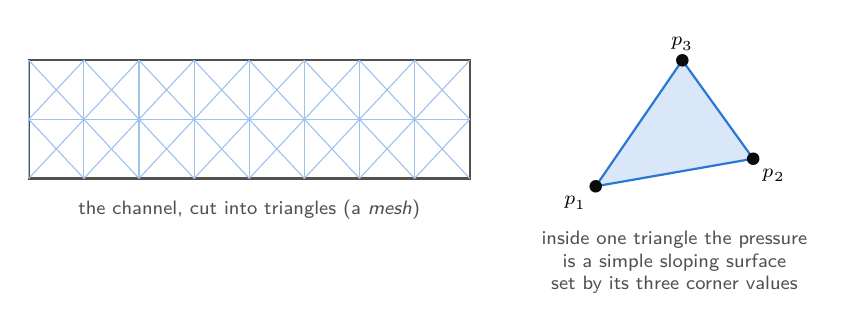
\begin{tikzpicture}[x=1cm,y=1cm,scale=1]
  \begin{scope}
  \draw[muted,thick] (0,0) rectangle (5.6,1.5);
  \foreach \i in {0,...,7}{
    \pgfmathsetmacro\x{\i*0.7}
    \draw[blue1!45] (\x,0)--(\x,1.5);
    \draw[blue1!45] (\x,0)--(\x+0.7,0.75);
    \draw[blue1!45] (\x,0.75)--(\x+0.7,1.5);
    \draw[blue1!45] (\x,0.75)--(\x+0.7,0);
    \draw[blue1!45] (\x,1.5)--(\x+0.7,0.75);
  }
  \draw[blue1!45] (0,0.75)--(5.6,0.75);
  \node[below,font=\scriptsize\sffamily,color=muted] at (2.8,-0.15)
       {the channel, cut into triangles (a \emph{mesh})};
  \end{scope}
  \begin{scope}[xshift=7.2cm,yshift=-0.1cm]
    \fill[blue1!18] (0,0)--(2,0.35)--(1.1,1.6)--cycle;
    \draw[blue1,thick] (0,0)--(2,0.35)--(1.1,1.6)--cycle;
    \foreach \p/\v in {(0,0)/$p_1$,(2,0.35)/$p_2$,(1.1,1.6)/$p_3$}{
      \node[circle,fill=ink,inner sep=1.6pt] at \p {};
    }
    \node[below left,font=\scriptsize] at (0,0) {$p_1$};
    \node[below right,font=\scriptsize] at (2,0.35) {$p_2$};
    \node[above,font=\scriptsize] at (1.1,1.6) {$p_3$};
    \node[below,font=\scriptsize\sffamily,color=muted,align=center]
         at (1,-0.45) {inside one triangle the pressure\\is a simple sloping surface\\
         set by its three corner values};
  \end{scope}
\end{tikzpicture}
\caption{The finite element method in one picture. Unknown ``the pressure
everywhere'' becomes unknown ``the pressure at each corner'', which is a finite
list of numbers a computer can solve for.}
\end{figure}

This converts an impossible calculus problem into a very large but ordinary
algebra problem:

\begin{equation}
\symbf{A}\,\symbf{p}=\symbf{b}
\end{equation}

\begin{center}\small
\begin{tabular}{ll}
\sym{\symbf{p}}{the list of unknown pressures, one per corner --- a few
thousand numbers}
\sym{\symbf{A}}{a big table encoding ``each corner must be consistent with its
neighbours''}
\sym{\symbf{b}}{what is driving the system --- here, the vibrating crystal underneath}
\end{tabular}
\end{center}

Solving simultaneous equations is something computers are extremely good at.
A typical run here has about 20\,000 unknowns and takes under a second.

\begin{plain}
Every finite element package in the world --- the free ones in this project and
the commercial ones costing tens of thousands per seat --- does this same thing.
They differ in convenience, geometry handling and support, not in the idea.
\end{plain}

\begin{figure}[h]
\centering
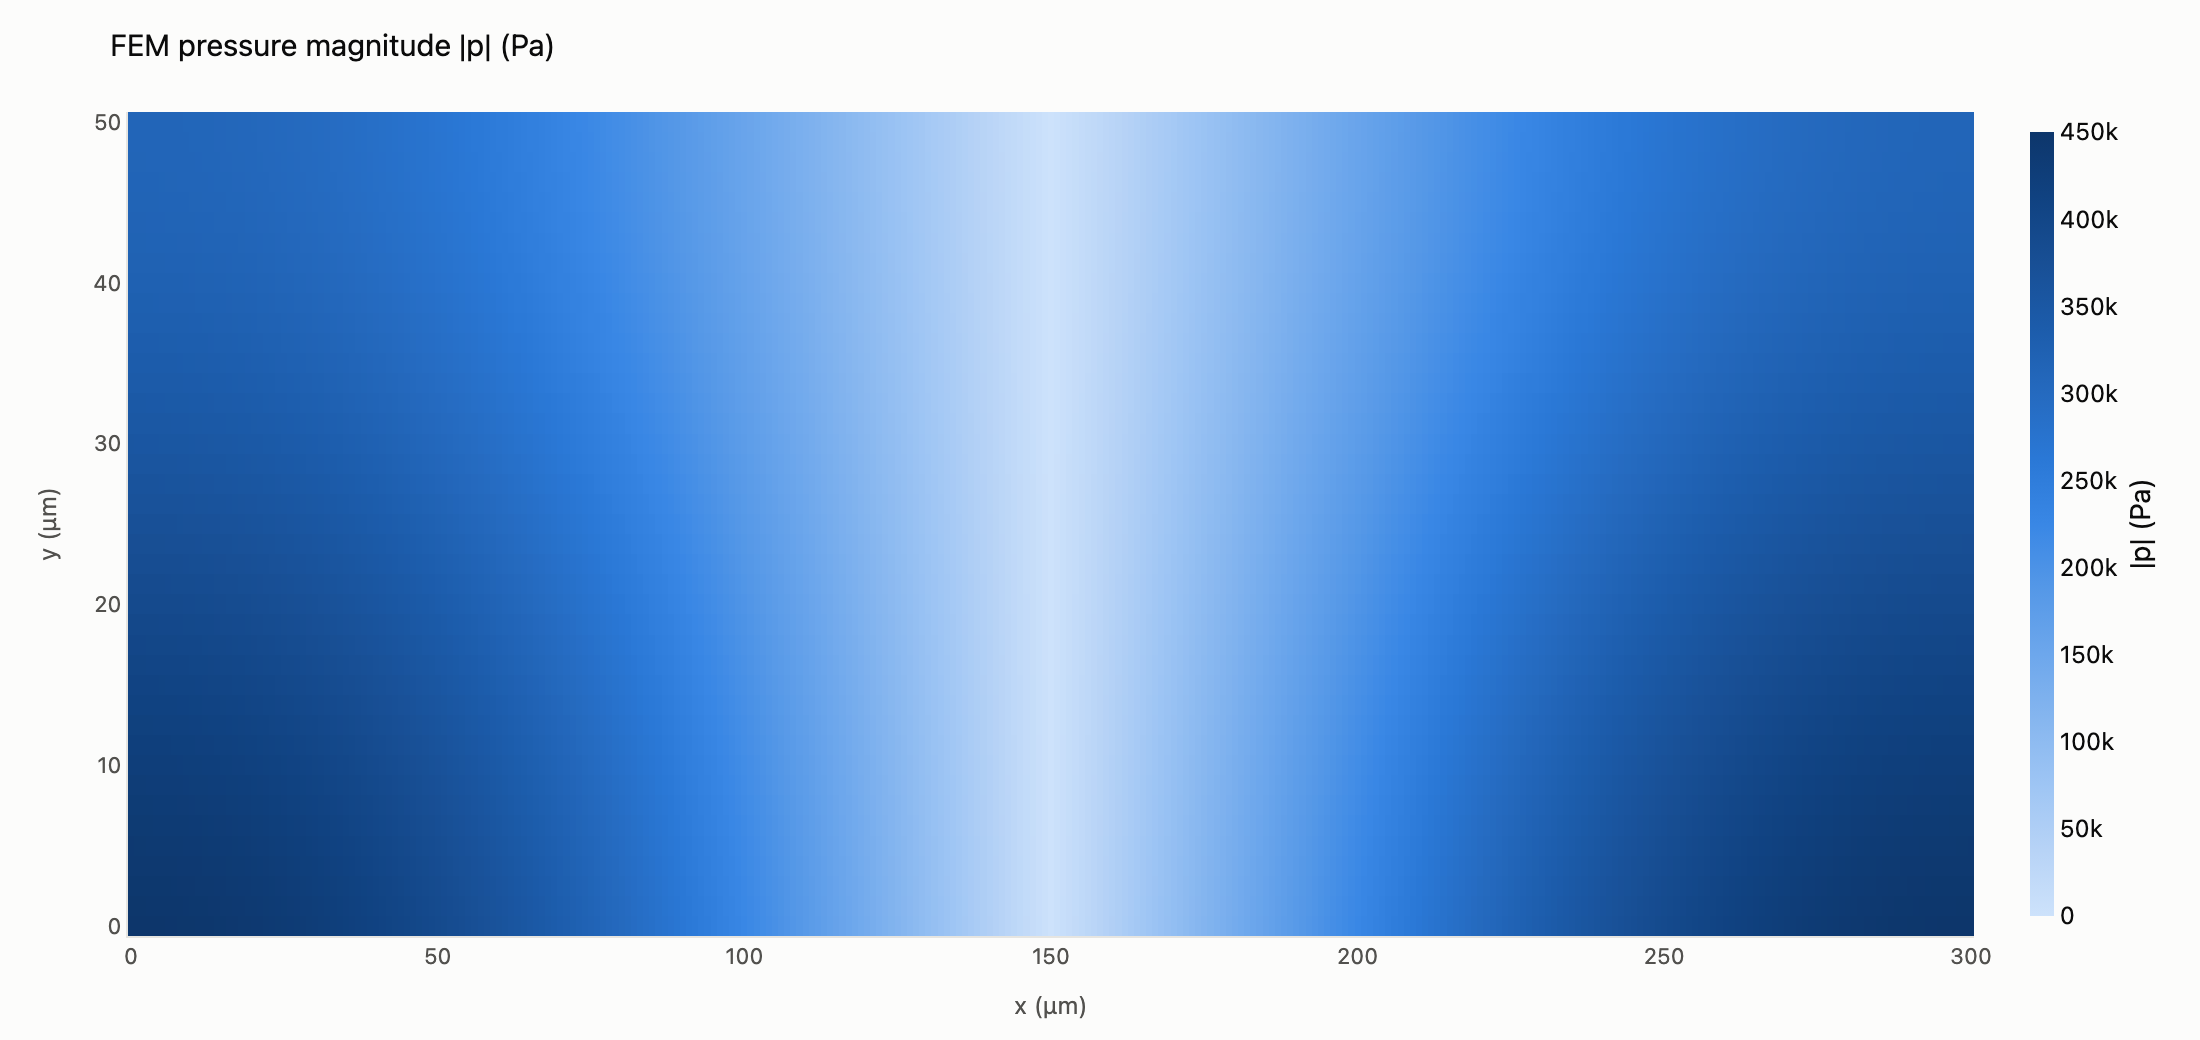
\includegraphics[width=0.9\textwidth]{../../assets/04_pressure_field.png}
\caption{The computed pressure field in the channel cross-section. Dark blue is
where the pressure swings hardest; the pale vertical stripe down the middle is
the node, where it never changes at all --- that is where the cells collect. The
channel is \SI{300}{\micro\meter} wide and \SI{50}{\micro\meter} tall. Notice
that the dark bands fade towards the top: the sound leaks out through the
ceiling, and that fading turns out to matter a great deal
(\S\ref{sec:limits}).}
\end{figure}

\section{Moving the cells}

With the force field known, each cell obeys equation~\eqref{eq:overdamped}:
its velocity is the water's velocity plus the acoustic push divided by the drag.
Written as a rule for how position changes with time:

\begin{equation}
\frac{d\symbf{x}}{dt}=\symbf{u}_f(\symbf{x})+\frac{\symbf{F}(\symbf{x})}{6\pi\mu r}
\end{equation}

This is an \textbf{ordinary differential equation}: a rule for the rate of
change, from which the computer reconstructs the path.

\begin{analogy}
It is dead reckoning. You know your speed and heading at every instant; step
forward a tiny amount of time, recompute, repeat. The only skill is choosing the
step size --- small enough to be accurate, large enough to finish. The software
lets the solver choose adaptively: small steps where the force changes quickly,
large steps where it does not.
\end{analogy}

All the cells are integrated as one system rather than one at a time, which is
why 800 cells take under a second.

\subsection*{One subtlety that cost real debugging time}

Cells reaching a wall must not leave the channel. The obvious fix is to zero out
any velocity pointing into the wall. Doing that made the simulation roughly a
hundred times slower.

The reason is that it makes the rule for velocity \emph{jump} discontinuously at
the wall. Adaptive solvers detect a jump by taking smaller and smaller steps
trying to resolve it, and effectively stall. The fix is to leave the rule smooth
and instead evaluate the force at the nearest point \emph{inside} the channel,
then clip the final path. Same physical answer, no discontinuity, full speed.

\begin{plain}
This is what most of the work in scientific computing actually is: not
inventing physics, but noticing that a mathematically harmless choice is
numerically catastrophic.
\end{plain}

\section{How do you know the code is right?}

This is the question that matters, and there is only one honest answer:
\textbf{compare against cases where you already know the answer.} A simulation
that has never been checked against anything is a picture, not a result.

\begin{center}\small
\begin{tabular}{p{5.3cm}p{5.0cm}r}
\toprule
\textbf{What is checked} & \textbf{Against what} & \textbf{Agreement} \\
\midrule
The electrical solver & the schoolbook formula for two parallel plates,
$Z=L/(\sigma A)$ & $10^{-9}$ \\[3pt]
The general force machinery & the hand-derived one-dimensional formula, on a
field where both apply exactly & $7\times10^{-6}$ \\[3pt]
The sound solver & the known shape of a standing wave in a box & $<2\,\%$ \\[3pt]
The flow formula & numerically integrating its own answer to recover the flow
rate it was given & $<10^{-3}$ \\[3pt]
The flow formula, again & the exact textbook result for an infinitely wide
channel (peak $=1.5\times$ mean) & 1.5047 \\[3pt]
The no-inertia shortcut & the full $F=ma$ calculation & $<10^{-3}$ \\[3pt]
The IC50 fitter & synthetic data with a planted answer & $<10^{-3}$ \\[3pt]
The tracking code & synthetic video with planted speed & $1\,\%$ \\
\bottomrule
\end{tabular}
\end{center}

Beyond numerical agreement, the test suite checks \emph{identities} --- things
that must be true regardless of the numbers:

\begin{itemize}
\item The force is exactly zero at nodes and at antinodes.
\item Doubling the loudness quadruples the force; doubling the volume doubles it.
\item Every cell in the body has $\Phi>0$; a fat droplet has $\Phi<0$.
\item The two rival definitions of $\Phi$ differ by exactly 3.
\item No cell is ever lost, duplicated, or found outside the channel.
\item Turning the sound off produces no separation at all.
\item Raising the flow rate always reduces capture.
\end{itemize}

\begin{plain}
Checking a number is weak evidence; checking a \emph{relationship} is strong
evidence. If someone changes the code and the force stops scaling with the cube
of the radius, a test fails immediately --- even though no specific number was
ever written down.
\end{plain}

There are 160 such checks. They run in 14 seconds and all pass, with no optional
software installed.

\subsection*{Convergence: is the mesh fine enough?}

A finite element answer depends on how finely you chop. If the answer keeps
changing as you refine, you are looking at your mesh, not at physics. The
symmetry error --- which must be zero in reality --- shrinks steadily:

\begin{center}\small
\begin{tabular}{rrr}
\toprule
\textbf{Mesh resolution} & \textbf{Peak force} & \textbf{Symmetry error} \\
\midrule
32  & \SI{109.60}{\pico\newton} & 0.118 \\
64  & \SI{106.70}{\pico\newton} & 0.021 \\
128 & \SI{106.23}{\pico\newton} & 0.009 \\
\bottomrule
\end{tabular}
\end{center}

Both columns settle down. That is what convergence looks like, and it is the
difference between a computed answer and a decorated guess.

% ============================================================================
\clearpage
\part*{Part VI --- The numbers, and what is wrong with them}
\addcontentsline{toc}{part}{Part VI --- The numbers and the limitations}

\section{Every number in the default experiment}

\begin{center}\small
\begin{tabular}{llr}
\toprule
\multicolumn{3}{l}{\textbf{What we choose (the device)}}\\
\midrule
Frequency & $f$ & \SI{6.632}{\mega\hertz} \\
Drive voltage & $V_{pp}$ & \SI{15}{\volt} \\
Channel width & $W$ & \SI{300}{\micro\meter} \\
Channel height & $H$ & \SI{50}{\micro\meter} \\
Active length & $L$ & \SI{2}{\milli\meter} \\
Flow rate & $Q$ & \SI{5}{\micro\liter\per\minute} \\
\midrule
\multicolumn{3}{l}{\textbf{What follows from those (the physics)}}\\
\midrule
SAW wavelength & $\lambda_{\text{SAW}}$ & \SI{600}{\micro\meter} \\
Node spacing & $\lambda_{\text{SAW}}/2$ & \SI{300}{\micro\meter} \\
Number of nodes in the channel & & 1, at the centre \\
Leak angle & $\theta_R$ & $22.1^\circ$ \\
Sound pressure & $p_0$ & \SI{0.45}{\mega\pascal} \\
Average flow speed & $\bar u$ & \SI{5.56}{\milli\meter\per\second} \\
Time in the device & $L/\bar u$ & \SI{0.36}{\second} \\
Channel Reynolds number & $\mathrm{Re}$ & 0.53 \\
Particle Reynolds number & $\mathrm{Re}_p$ & 0.15 \\
\midrule
\multicolumn{3}{l}{\textbf{What each cell feels}}\\
\midrule
Peak force on a tumour cell & & \SI{129.6}{\pico\newton} \\
Peak force on a red cell & & \SI{5.4}{\pico\newton} \\
Force ratio & & $24\times$ \\
Speed ratio (force $\div$ drag) & & $7.4\times$ \\
Tumour cell's top speed sideways & & \SI{858}{\micro\meter\per\second} \\
\midrule
\multicolumn{3}{l}{\textbf{What comes out}}\\
\midrule
Recovery (tumour cells collected) & & $100\,\%$ \\
Purity (of what was collected) & & $94.3\,\%$ \\
Enrichment over the input ratio & & $1.9\times$ \\
\bottomrule
\end{tabular}
\end{center}

\begin{plain}
\SI{129.6}{\pico\newton} is a piconewton --- a trillionth of a newton. It is
roughly the force gravity exerts on a single bacterium. It is also about ten
times the force a molecular motor inside your cells produces, and about a
hundredth of the force needed to break a chemical bond. It is small enough not
to damage the cell and large enough to steer it. That window is why this
technique exists at all.
\end{plain}

\begin{figure}[h]
\centering
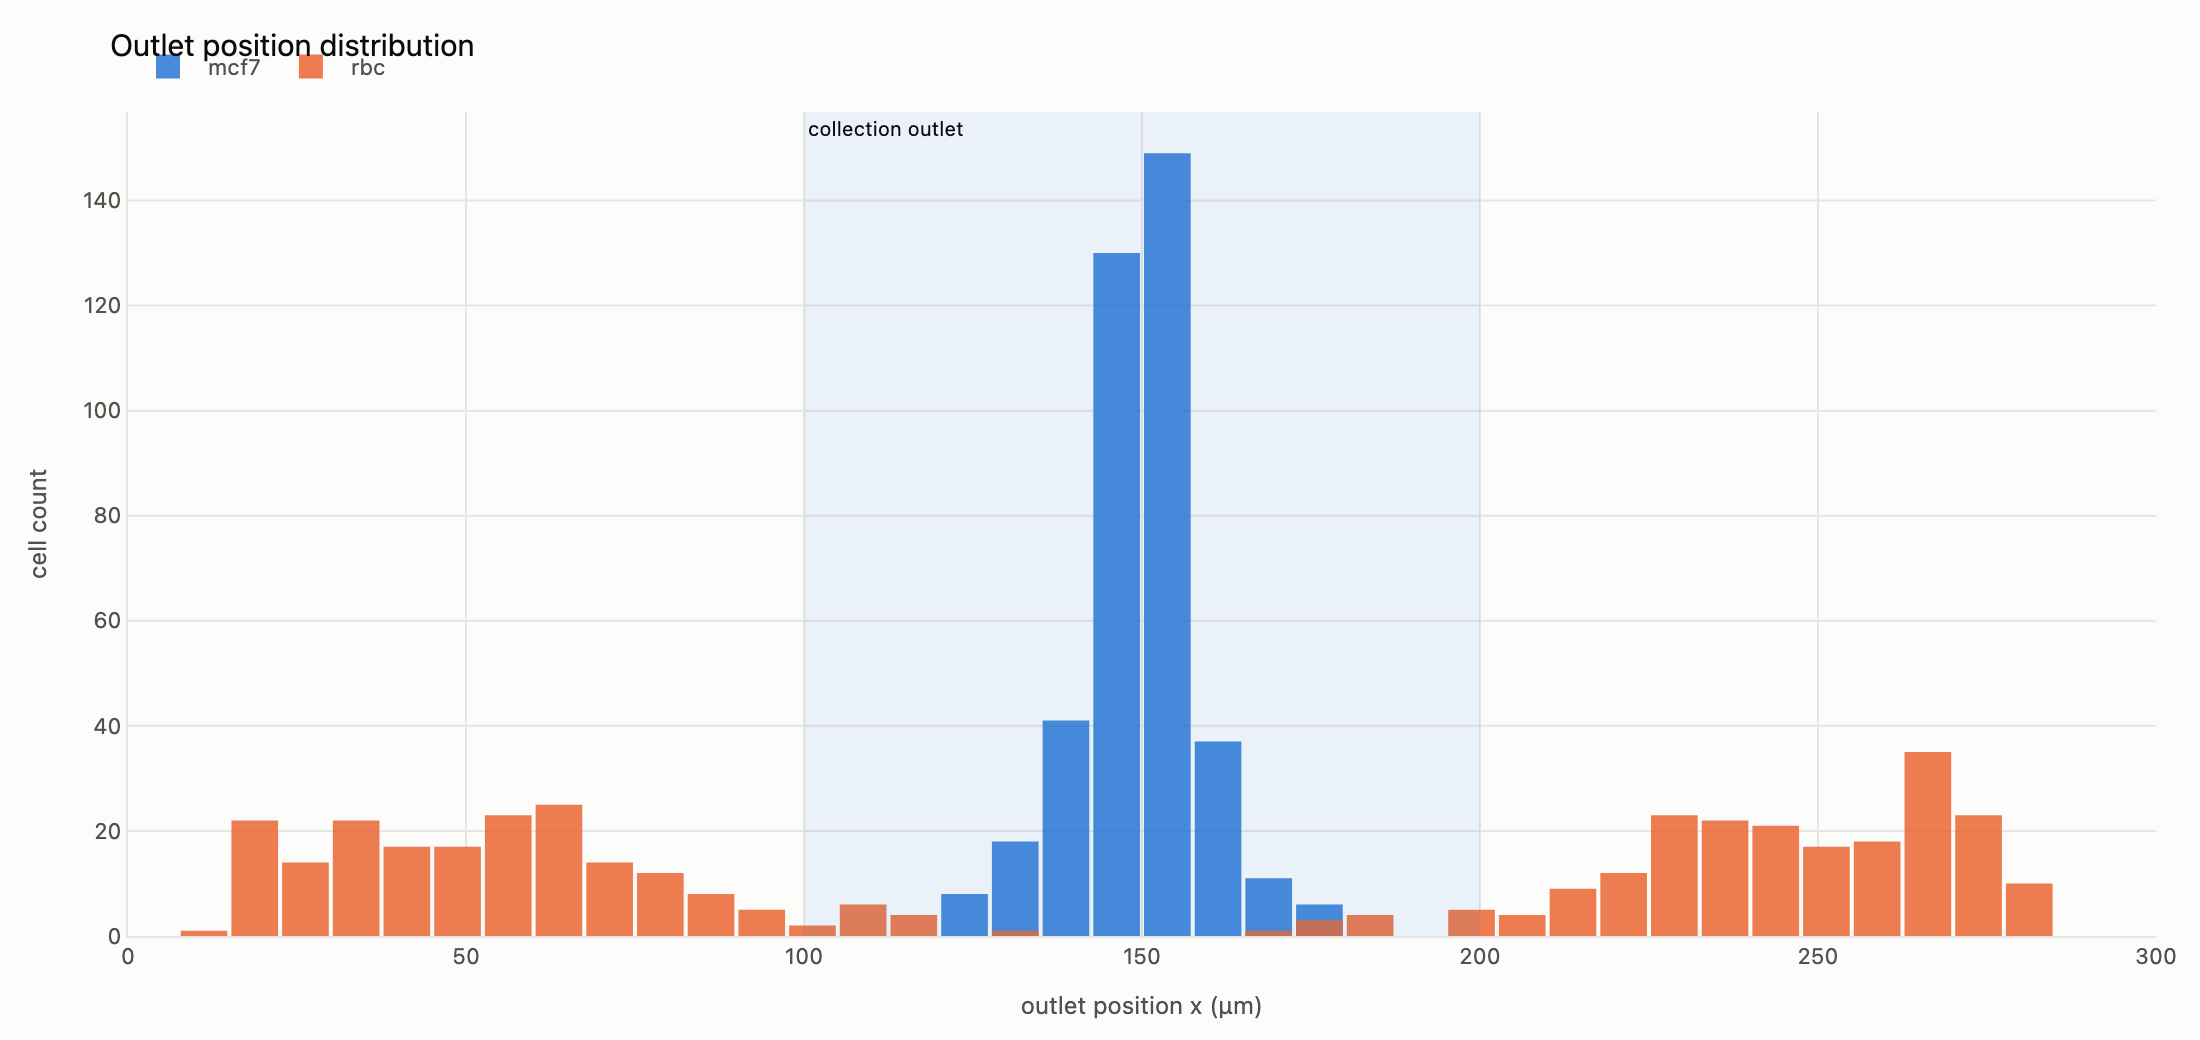
\includegraphics[width=0.86\textwidth]{../../assets/02_outlet_histogram.png}
\caption{Where the cells come out. Blue tumour cells pile into the central
collection outlet; orange red cells stay near the walls where they started.
The small orange overlap in the middle is the 6\,\% of red cells that were
unusually large, or started closer to the centre, and it is the reason purity
is 94\,\% rather than 100\,\%.}
\end{figure}

\subsection*{On a realistic blood sample}

The demonstration above uses a 50:50 mixture, which is convenient and not
realistic. With tumour cells spiked at 1\,\% into a full blood background of red
cells, white cells and platelets, the same device gives:

\begin{center}\small
\begin{tabular}{lr}
\toprule
Recovery & $100\,\%$ \\
Purity of the collected fraction & $10\,\%$ \\
\textbf{Enrichment} & $\mathbf{10\times}$ \\
\bottomrule
\end{tabular}
\end{center}

Enrichment is the number that matters clinically: the sample handed to the next
stage is ten times richer in tumour cells than the blood that went in, with none
of them lost. Real workflows chain several such stages.

\section{What is assumed, and what is wrong}
\label{sec:limits}

This is the most important section in the document.

\subsection*{The single biggest assumption}

Nothing in this software predicts how loud the sound is for a given drive
voltage. That calculation requires solving the full electrical-mechanical
behaviour of the crystal and the electrode pattern, which is a separate and
harder problem.

Instead there is a straight-line calibration --- 15 volts gives
\SI{0.45}{\mega\pascal} --- which is inside the range published for devices of
this kind, and is labelled in the source code as an assumption in capital
letters. It scales every force in the simulation.

\begin{plain}
If you build this device, do not trust the voltage. Measure the pressure ---
by tracking calibration beads of known properties and fitting how fast they
move --- and put that measured number in. The software accepts it directly for
exactly this reason.
\end{plain}

\subsection*{The simple model is optimistic}

The one-dimensional formula, equation~\eqref{eq:force}, applies the sound
strength measured at the crystal surface to cells at \emph{every} height in the
channel. The real field weakens with height as it leaks out through the ceiling:

\begin{center}\small
\begin{tabular}{rrl}
\toprule
\textbf{Height above the crystal} & \textbf{Sideways force} & \\
\midrule
\SI{0}{\micro\meter}  & \SI{106.7}{\pico\newton} & (the value the simple model uses everywhere) \\
\SI{10}{\micro\meter} & \SI{88.5}{\pico\newton}  & \\
\SI{20}{\micro\meter} & \SI{64.9}{\pico\newton}  & \\
\SI{30}{\micro\meter} & \SI{41.9}{\pico\newton}  & \\
\SI{40}{\micro\meter} & \SI{25.6}{\pico\newton}  & \\
\SI{50}{\micro\meter} & \SI{19.9}{\pico\newton}  & (at the ceiling) \\
\midrule
\multicolumn{2}{l}{\textbf{Average across the channel}} & \textbf{53\,\% of the surface value} \\
\bottomrule
\end{tabular}
\end{center}

A cell drifting near the ceiling feels a fifth of the push the simple model
assumes. So the simple model is a \textbf{best case}, and the finite element
model is the realistic one. Both ship, the difference is measured by a script
that anyone can run, and the test suite forbids the finite element result from
ever coming out more optimistic than the simple one.

\subsection*{Things left out entirely}

\begin{center}\small
\begin{tabular}{p{4.3cm}p{10.3cm}}
\toprule
\textbf{Left out} & \textbf{Why, and when it will bite you} \\
\midrule
\textbf{Acoustic streaming} &
Sound loses a little energy at the walls, which stirs the liquid into slow
steady swirls. This stirring does \emph{not} depend on particle size, while the
sorting force scales with $r^3$. Below a critical radius --- about
\SI{1}{\micro\meter} in water at these frequencies --- the stirring wins and
particles are mixed rather than sorted. Irrelevant for \SI{9}{\micro\meter}
tumour cells; fatal for bacteria or platelets. \\[4pt]
\textbf{Cells pushing each other} &
Two cells in the same sound field scatter onto each other and attract. This is
why acoustophoresis videos show cells forming chains. Ignored because it costs
$N^2$ computation and only matters above roughly $10^6$ cells per mL. \\[4pt]
\textbf{Vertical forces} &
The model computes them but does not apply them by default. In a genuine
channel, cells are held at a stable height by lift forces this two-dimensional
model does not include; without those, cells pile against a wall where the flow
is zero and never leave. Turning it on makes the failure visible rather than
hidden --- the results table reports that cells failed to exit. \\[4pt]
\textbf{Cells being squishy} &
A cell is treated as a rigid sphere of uniform jelly. Real cells deform, and
deformability is itself a cancer marker. A different physics entirely. \\[4pt]
\textbf{The membrane and nucleus} &
For sound, the cell is one uniform blob. For the impedance instrument, the
membrane is modelled explicitly, because there it is the whole effect. \\
\bottomrule
\end{tabular}
\end{center}

\subsection*{Where the model is being stretched even when it works}

The whole acoustic theory assumes the cell is much smaller than the sound
wavelength. The measure of this is $k a$, roughly ``how many wavelengths across
is the cell''. The usual limit is $ka < 0.1$.

\begin{center}\small
\begin{tabular}{rrl}
\toprule
\textbf{Frequency} & $ka$ \textbf{for a \SI{9}{\micro\meter} cell} & \\
\midrule
\SI{6.632}{\mega\hertz} & 0.39 & \textbf{beyond the textbook limit --- warned} \\
\SI{20}{\mega\hertz}    & 1.06 & \textbf{badly beyond it --- warned loudly} \\
\bottomrule
\end{tabular}
\end{center}

\begin{warnbox}
The default operating point is already outside the strict validity of the theory
it uses. This is not a flaw introduced here --- the published experimental
literature on acoustic tumour-cell separation operates in the same regime, and
the theory is known to over-predict the force there.

The software's response is to compute the number and print a warning naming the
reference, on every run, rather than to stay quiet. A model that tells you when
it is being used outside its range is more useful than one that is silently
narrower.
\end{warnbox}

\subsection*{Where the numbers come from}

Every physical constant in the software carries either a published reference
(a DOI) or an explicit label saying it is an assumption together with the reason.
There is no third category, and an automated test refuses to let anyone add one.

Of the 65 material values, 27 have published sources and 38 are flagged
assumptions. Running \texttt{biosim materials} prints the 38, with the reason for
each. That list is exactly what a methods section ought to disclose.

\begin{plain}
The point is not that assumptions are bad. It is that a reader should be able to
find out, in one command, which numbers were measured by someone and which were
chosen by the author --- rather than having all 65 presented with the same
authority.
\end{plain}

% ============================================================================
\clearpage
\section{The whole thing on one page}

\begin{enumerate}[leftmargin=*,itemsep=6pt]
\item \textbf{The problem is a needle in a haystack.} One tumour cell among five
billion blood cells, and it must survive the search.

\item \textbf{The handle is size.} Tumour cells are about three times wider than
red blood cells, and nothing a cell can do hides that.

\item \textbf{Sound provides a gentle, invisible landscape.} Two surface waves
sent from opposite sides of a chip make a standing pattern with quiet lines and
loud lines. Cells roll downhill towards the quiet lines.

\item \textbf{The push grows with volume; the resistance grows with width.} So
sideways speed scales with radius squared. A cell three times wider moves about
ten times faster. \emph{This single fact is the device.}

\item \textbf{Everything else is timing.} Cells spend 0.36 seconds in the sound
field. Tumour cells reach the middle in that time; red cells do not. Tap the
middle outlet.

\item \textbf{The maths is one equation with five factors:} how loud, how big
the cell, how different from water, how tight the pattern, and where the cell
sits relative to the quiet line.

\item \textbf{The computation is triangles and dead reckoning.} Chop the
channel into triangles to find the sound field; then step each cell forward in
tiny time increments.

\item \textbf{The credibility is in the checking.} 160 automated tests compare
against hand-solvable cases, verify relationships that must hold regardless of
numbers, and confirm the answer stops changing as the mesh is refined.

\item \textbf{The honesty is in the warnings.} The model announces when it is
outside its validity, when the operating point produces the wrong number of
quiet lines, and which of its inputs were assumed rather than measured.

\item \textbf{The same skeleton runs three more instruments} --- impedance
monitoring, cell counting, cell tracking --- because they share the same core:
describe the experiment, validate it, solve it, save it, plot it.
\end{enumerate}

\vfill

\begin{center}
\begin{minipage}{0.9\textwidth}
\small\color{muted}
\textbf{A closing note on what simulation is for.} None of this replaces an
experiment. What it does is let you find out, in seconds and at no cost, that
\SI{20}{\mega\hertz} in a \SI{300}{\micro\meter} channel gives you three
collection stripes instead of one --- rather than finding out after fabricating
the chip. That is the whole value proposition: mistakes made in software are
cheap.
\end{minipage}
\end{center}

% ============================================================================
\clearpage
\appendix
\section{Every symbol, in one table}

\begin{center}\small
\begin{tabular}{cll}
\toprule
\textbf{Symbol} & \textbf{Name} & \textbf{Plain meaning} \\
\midrule
$r$ & radius & how big the cell is \\
$V_c$ & volume & $\tfrac43\pi r^3$ \\
$\rho_p,\rho_f$ & density & how heavy the cell / the water is, per unit volume \\
$\kappa_p,\kappa_f$ & compressibility & how easily the cell / the water squeezes \\
$\mu$ & viscosity & how thick the liquid is \\
$c$ & speed of sound & how fast the pattern travels \\
$f$ & frequency & how many wiggles per second \\
$\lambda$ & wavelength & distance between wiggles \\
$k$ & wavenumber & $2\pi/\lambda$; wavelength, upside down \\
$p_0$ & pressure amplitude & how loud \\
$\Phi$ & contrast factor & which way the cell goes, and how strongly \\
$f_1,f_2$ & scattering terms & the stiffness part and the weight part of $\Phi$ \\
$U$ & Gor'kov potential & the height of the invisible landscape \\
$F_r$ & radiation force & the sideways push from the sound \\
$F_d$ & drag force & the water's resistance \\
$\mathrm{Re}$ & Reynolds number & whether the liquid coasts (it does not, here) \\
$Q$ & flow rate & how fast liquid is pumped in \\
$Z$ & impedance & electrical resistance for alternating current \\
$\mathrm{CI}$ & Cell Index & how covered the electrode is \\
$\mathrm{IC}_{50}$ & half-maximal dose & the drug concentration that kills half \\
$\mathrm{MSD}$ & mean-squared displacement & how far a cell wanders \\
$\alpha$ & MSD exponent & 1 = random wandering, 2 = walking somewhere \\
\bottomrule
\end{tabular}
\end{center}

\section{Units, for people who do not think in them}

\begin{center}\small
\begin{tabular}{lll}
\toprule
\textbf{Unit} & \textbf{Size} & \textbf{Something that size} \\
\midrule
metre & 1 & a long stride \\
millimetre (mm) & one thousandth & thickness of a coin \\
micrometre (µm) & one millionth & a red blood cell is 8 across \\
nanometre (nm) & one billionth & a cell membrane is 5 thick \\
\midrule
newton (N) & 1 & the weight of an apple \\
piconewton (pN) & one trillionth & \textbf{the forces in this document} \\
\midrule
pascal (Pa) & 1 & very small pressure \\
kilopascal (kPa) & one thousand & atmospheric pressure is 101 \\
megapascal (MPa) & one million & \textbf{our sound pressure is 0.45} \\
\midrule
hertz (Hz) & 1 per second & a slow heartbeat \\
megahertz (MHz) & one million per second & \textbf{our frequency is 6.6} \\
\midrule
litre (L) & 1 & a carton of milk \\
microlitre (µL) & one millionth & a small droplet; \textbf{we pump 5 per minute} \\
\bottomrule
\end{tabular}
\end{center}

\section{Where each idea came from}

The physics here is not new. This software implements published results; the
contribution is putting them together in open code with the assumptions labelled.

\begin{center}\small
\begin{tabular}{p{5.0cm}p{9.5cm}}
\toprule
\textbf{Idea} & \textbf{Source} \\
\midrule
The force on a small particle in a sound field &
Gor'kov (1962); modern derivation in Bruus, \emph{Lab on a Chip} \textbf{12}:1014
(2012), \texttt{doi:10.1039/c2lc21068a} \\[4pt]
Node spacing is set by the crystal, not the liquid &
Shi et al., \emph{Lab on a Chip} \textbf{9}:3354 (2009),
\texttt{doi:10.1039/b910595f} \\[4pt]
Sorting tumour cells this way &
Li et al., \emph{PNAS} \textbf{112}:4970 (2015),
\texttt{doi:10.1073/pnas.1504484112} \\[4pt]
Drag on a sphere in slow flow &
Stokes (1851); Batchelor, \texttt{doi:10.1017/CBO9780511800955} \\[4pt]
Flow in a rectangular channel &
White, \emph{Viscous Fluid Flow}; Bruus, \emph{Theoretical Microfluidics} \\[4pt]
Measuring cells with electrodes &
Giaever \& Keese, \emph{PNAS} \textbf{88}:7896 (1991),
\texttt{doi:10.1073/pnas.88.17.7896} \\[4pt]
Following particles between video frames &
Crocker \& Grier, \emph{J.\ Colloid Interface Sci.} \textbf{179}:298 (1996),
\texttt{doi:10.1006/jcis.1996.0217} \\[4pt]
Cell motion as a persistent random walk &
Selmeczi et al., \emph{Biophysical Journal} \textbf{89}:912 (2005),
\texttt{doi:10.1529/biophysj.105.061150} \\[4pt]
Acoustic streaming, and when it takes over &
Muller et al., \emph{Lab on a Chip} \textbf{12}:4617 (2012),
\texttt{doi:10.1039/c2lc40612h} \\
\bottomrule
\end{tabular}
\end{center}

\vspace{1cm}
\begin{center}
\small\color{muted}
The complete list of sources, including every material constant and every value
that was assumed rather than measured, is in \texttt{docs/physics.md} and can be
printed with \texttt{biosim materials}.
\end{center}

\end{document}
